\documentclass[a4paper]{book} 

% Engine Specific Packages
% pdftex
\ifx\pdfmatch\undefined
\else
   \usepackage[T1]{fontenc}
   \usepackage[utf8]{inputenc}
   \usepackage[italian]{babel}
\fi
% luatex
\ifx\directlua\undefined
\else
   \usepackage{fontspec}
   \usepackage[italian]{poliglossia}
\fi

\usepackage{enumitem,graphicx,hyphenat,titlesec,titletoc,xcolor,url}
\usepackage{amsmath,amsthm,amssymb,amsfonts}
\allowdisplaybreaks
\usepackage[babel=true,final]{microtype} 
\usepackage[heightrounded,showframe=false,paper=a4paper,margin=1in]{geometry}
\usepackage{wrapfig}
\usepackage{array}
\usepackage{tabularx}
\usepackage{boiboites}
\usepackage{pythontex}
\usepackage{etoolbox}
\usepackage{needspace}
\usepackage{fancyhdr}
\usepackage{register}

\pagestyle{fancy}
\fancyhf{}
\fancyhead[RE]{\footnotesize \textsf{\leftmark}}
\fancyhead[LO]{\footnotesize \textsf{\rightmark}}
\fancyhead[LE,RO]{\footnotesize \textsf{\thepage}}
%\fancyhead[RE,LO]{\textsf{\thepage - \rightmark}}

\usepackage{caption}

%-----------------------

\usepackage{epigraph} 
\setlength{\epigraphwidth}{0.7\textwidth}
\renewcommand{\epigraphsize}{\small}

\makeatletter 
\renewcommand\maketitle{
\begin{titlepage} \vspace*{\stretch{1}}
 \begin{center} {\Huge \@title \par}% 
	 \vspace{5em}% 
	 {\LARGE \@author \par}%
	 \vspace{1.5em} {
	 \large \emph{\@date} \par}% 
	 \end{center}%
 \vspace*{\stretch{1}} 
\end{titlepage}} 
\makeatother

\definecolor{titlecolor}{rgb}{0,0,0.5}
\definecolor{grey60}{rgb}{0.7,0.7,0.7}
\definecolor{shadethmcolor}{HTML}{EDF8FF}
\definecolor{shaderulecolor}{HTML}{45CFFF}

%\pagestyle{fancy}
%\renewcommand{\headrulewidth}{0.01pt}
%\lhead{}
%\renewcommand{\chaptermark}[1]{%
%\markboth{\chaptername \ \thechapter.\ #1}{}}

\titleformat{\chapter}[display]
            {\raggedright\normalfont\Large\color{titlecolor}}
			{\chaptertitlename\ \thechapter}{0pt}{\Huge}[\vspace{5pt}\titlerule]
\titleformat{\section}
			{\raggedright\normalfont\Large\bfseries\color{titlecolor}}
			{\thesection}{1ex}{}
\titleformat{\subsection}
			{\raggedright\normalfont\large\bfseries\color{titlecolor}}
			{\thesubsection}{1ex}{}
\titleformat{\paragraph}[runin]
			{\normalfont\normalsize\bfseries}{\theparagraph}{1em}{}


\newcommand{\uchapter}[1]{\chapter*{#1}\phantomsection\addcontentsline{toc}{chapter}{#1}}
\newcommand{\usection}[1]{\section*{#1}\phantomsection\addcontentsline{toc}{section}{#1}}


%---- TOC ----

\contentsmargin{7mm}

\titlecontents{part}
              [0mm]
              {\addvspace{7mm}\Large\bfseries\color{titlecolor}}
              {}
              {Part }
              {}

\titlecontents{chapter}
              [6mm]
              {\addvspace{4mm}\bfseries}
              {\contentslabel{6mm}}
              {\hspace*{-6mm}}
              {\titlerule[0pt]\contentspage}
              [\addvspace{2mm}]

\titlecontents{section}
              [15mm]
              {}
              {\contentslabel{9mm}}
              {\hspace*{-9mm}}
              { \titlerule*[0.7pc]{.}\contentspage}

\titlecontents{subsection}
              [27mm]
              {}
              {\contentslabel{12mm}}
              {\hspace*{-12mm}}
              { \titlerule*[0.7pc]{.}\contentspage}
%--------------------



\pagestyle{plain} 
\pagenumbering{alpha} 
\titlespacing*{\chapter}{0pt}{0pt}{40pt}

\hyphenation{rap-pre-sen-ta-zio-ne}

\newboxedtheorem[
	boxcolor = shaderulecolor, % red!50!black, 
	background= shadethmcolor, %blue!5, 
	titlebackground= blue!20,
	titleboxcolor=black]{thm}{Teorema}{thmCounter} 
%\break if fewer than 5\baselineskip is available on page	
\AtBeginEnvironment{thm}{\Needspace{5\baselineskip}} 
	
\newboxedtheorem[
	boxcolor = orange, 
	background=blue!5, 
	titlebackground=blue!20,
	titleboxcolor=black]{defn}{Definizione}{defCounter} 
\newboxedtheorem[
	boxcolor = black, 
	background=blue!5, 
	titlebackground=blue!5,
	titleboxcolor=black]{observe}{Osservazione}{obsCounter} 

%\newboxedtheorem[
%	boxcolor = black, 
%	background=blue!2, 
%	titlebackground=blue!20,
%	titleboxcolor=black,
%	size=0.94\textwidth]{ex}{Esempio}{exCounter} 

%\theoremstyle{definition}
%\newtheorem{ex}{Esempio}

%\usepackage[framemethod=default]{mdframed}
\usepackage{tikz}
\usepackage[framemethod=tikz]{mdframed}

\global\mdfdefinestyle{lemma}{%
	linecolor=blue!20,linewidth=1.5pt,
	skipabove=3\parskip,skipbelow=3\parskip,
	topline=false,rightline=false,bottomline=true
}
\newcounter{excounter}
\newenvironment{ex}[1][]{%
 \refstepcounter{excounter}%
  \ifstrempty{#1}%
  {\begin{mdframed}[style=lemma]
  {\bfseries{Esempio~\theexcounter:}}
  \relax}
  {\begin{mdframed}[style=lemma]
  {\bfseries{Esempio~\theexcounter}} (#1){\bfseries{:}}\relax%
}}{\end{mdframed}}

\renewenvironment{proof}[1][]{%
  \ifstrempty{#1} {\begin{mdframed}[linecolor=blue!20,linewidth=1.5pt,topline=false,
  rightline=false,bottomline=false]{\itshape{Dimostrazione: }}\relax}  {\begin{mdframed}[linecolor=blue!20,linewidth=1.5pt,topline=false,rightline=false,bottomline=false]{\itshape{Dimostrazione: }} (#1)\relax}}
  {\hfill\qed\end{mdframed}}


\usepackage{setspace} 
\setstretch{1.03} 
\setlength{\parskip}{0.2em}

\usepackage{hyperref}   % last package
\hypersetup{
	pdftitle={Note per il Corso di Programmazione},
	pdfauthor={Antonio Caruso}} 
\hypersetup{ 
	colorlinks=true, 
	linkcolor=black,
	citecolor=black, 
	filecolor=black, 
	urlcolor=black
}

% ---- Front matter ---- 

\title{Note per il Corso di Programmazione}
\author{Antonio Caruso\\[2ex] 
 {\normalsize Dipartimento di Matematica e Fisica '\emph{Ennio De Giorgi}'\\   
              Palazzo Fiorini\\[2ex] 
 \url{mailto://antonio.caruso@unisalento.it}\\
 \url{http://bilbo.unisalento.it/antonio}}} 
\date{Settembre 2015} 
\pagestyle{plain} 

\clubpenalty=10000 \widowpenalty=10000 \overfullrule=1mm

\newcommand{\nota}[1]{\marginpar[{\raggedleft\small\sffamily #1\\}]{%
 								 {\raggedright\small\sffamily #1\\}}}
\newcommand{\Mod}[1]{\ \text{mod}\ #1}

\includeonly{numeri,hardware,algoritmi}

\begin{document}

\frontmatter

\hypersetup{pageanchor=false}
\pagestyle{empty} 
\maketitle
\tableofcontents

\uchapter{Prefazione}

Queste Note fanno parte del materiale didattico per il corso di Programmazione presso l'Università degli Studi del Salento (Laurea Triennale in Matematica). 
Il corso prevede 6 crediti ETCS, ogni settimana vi sono di norma 2 ore di lezione e 2 ore di lezione/esercitazione presso il laboratorio di calcolo del Dipartimento.
Gli argomenti inclusi sono:
\begin{itemize}
\item \textbf{Rappresentazione dell'Informazione} all'interno del Calcolatore, con un enfasi particolare per la parte numerica.
\item \textbf{Architettura del Calcolatore}: Logica digitale, Circuiti Combinatorici/Sequenziali, Modello di Calcolo di Von Neumann. Architettura e Funzionamento del sistema centrale CPU-RAM.
\item \textbf{Algoritmi e Modelli di Calcolo}: Concetti, Modelli e Formalizzazioni della nozione di Algoritmo/Programma.  
\end{itemize}
Non è richiesta conoscenza preliminare sugli argomenti trattati nel corso. E' necessaria una conoscenza di base di Matematica Discreta e di Algebra.

Si ringraziano in anticipo coloro che, qualora trovassero delle inesattezze o errori nelle note, vogliano cortesemente segnalarmele via email, o direttamente a lezione.
\vspace*{\stretch{1}}
\section*{License}
\begin{samepage}
This work is licensed under the \emph{Creative Commons Attribution--ShareAlike 3.0 Unported License}. To view a copy of this license, visit
\begin{center}
    \url{http://creativecommons.org/licenses/by-sa/3.0/}
\end{center}
\end{samepage}

\mainmatter
\pagestyle{fancy} 

%\hypersetup{pageanchor=true} 

\newgeometry{vmargin=30mm, right=1.9in, marginparsep=3.5mm, footskip=15mm}

%!TEX root = note.tex

\chapter{Rappresentazione dei Numeri}

\epigraph{I do hate sums!! There is no greater mistake than to call arithmetic
an exact science. There are $\ldots$ hidden laws of Number which it requires a
mind like mine to perceive. For instance, if you add a sum from the bottom up,
and then again from the top down, the result is always different!}{ -
\textsc{M. P. LA TOUCHE} (1878)}

\epigraph{Vedete, non esiste nulla (amati studenti in Matematica) che sia così
fastidioso nella pratica matematica, e più molesto che dover calcolare
moltiplicazioni, divisioni, e radici quadrate o cubiche di numeri molto grandi.
A parte la noia e lo spreco di tempo, queste sono spesso soggette a errori
scivolosi. Ho cominciato a considerare nella mia mente, con quale arte io possa
rimuovere tali ostacoli.} { - \textsc{JOHN NEPAIR [Napier] (1916)}}

\section[Numeri Interi]{Numeri Interi}

Il primo approccio con la Matematica è \emph{contare}. Il contare porta alla
definizione dei numeri interi, attualmente scritti attraverso l'uso di una
\emph{notazione posizionale decimale} che come vedremo è stata introdotta in
Europa intorno al A.D. $1202$\footnote{Quindi per migliaia di anni il modo con
cui si pensava ad i numeri, li si scriveva e sopratutto si faceva Aritmetica è
stato molto diverso da come noi siamo abituati a fare sin da piccoli.} da parte
di Leonardo Pisano (detto il Fibonacci). Gli Interi e le operazioni elementari
tra essi, come somma, sottrazione, moltiplicazione e divisione sono studiati in
quella parte della matematica chiamata \emph{Aritmetica}; Nonostante il lettore
possa trovare strano dover rivedere concetti che ritiene assodati, vedremo come
l'Aritmetica meriti senz'altro un ulteriore approfondimento.

Queste note introdurranno una diversa prospettiva sul perché scriviamo i numeri
in decimale. Vedremo come la scelta di una rappresentazione numerica è
strettamente legata al modo con cui svolgiamo abitualmente le operazioni
aritmetiche, cioè gli \emph{algoritmi} usati per il calcolo di somma,
sottrazione, etc. Questi aspetti sono di interesse sia per comprendere
all'interno del corso di Programmazione come viene rappresentata l'informazione
dentro il computer, sia per chi dovrà svolgere attività didattica nelle scuole
elementari; evidenziando la natura essenzialmente \emph{algoritmica}
dell'Aritmetica.

Siamo interessati in particolare allo studio della \emph{rappresentazione} dei
numeri. In questa prospettiva dobbiamo chiaramente sottolineare la differenza
tra due entità: un numero, inteso astrattamente come \emph{valore} e la sua
\emph{rappresentazione} (o \emph{numerale}) intesa come sequenza di segni che
servono appunto a scrivere o comunicare un certo valore. Cominciamo quindi,
\marginnote{rappresentazione vs.\\ valore} con il distinguere un valore
numerico, ad esempio l'intero $1234$, da una delle sue tante possibili
\emph{rappresentazioni}, termine che vuol indicare \emph{il modo in cui
scriviamo} quel valore. Noi scriviamo (e pensiamo) i numeri allo stesso modo,
usando un sistema posizionale \emph{decimale} pertanto il modo più comune di
scrivere $1234$ è ovviamente: \textsf{'1234'}\footnote{le due scritture sono
diverse per enfatizzare che $1234$ è il valore, ed \textsf{'1234'} solo un modo
particolare per scrivere tale valore.}, ma lo stesso numero sarebbe stato
scritto come \textsf{'MCCXXXIV'} se vivessimo nell'antica Roma. Una
rappresentazione numerica è una serie di convenzioni più o meno formalizzabili
che descrivono come si \emph{scrivono} i numeri, cioè una serie di regole
\emph{'sintattiche'} che possono variare nel tempo e nello spazio.

La rappresentazione posizionale, ci consente di scrivere qualunque numero
(naturale) come una \emph{stringa}\footnote{sequenza di caratteri giustapposti}
di \emph{cifre} (\emph{digit} in inglese). Vale il seguente Teorema:


%%% Definizione Rappresentazione Posizionale


\begin{thm}[Rappresentazione dei numeri Naturali in base $B$] Sia $B>1$ un
intero che chiameremo \emph{base (o radice)} della rap\-presentazione, e
$\mathcal{C} = \{ c_0, c_1, \ldots c_{B-1} \}$ un insieme di simboli distinti
dette \emph{cifre della rappresentazione} (in inglese \emph{digit}). Ogni cifra
è associata ad un valore intero tra $0$ e $B-1$.\bigskip

Allora $\forall n \in \mathbb{N}$, esiste ed è unica la sequenza di cifre:
$(c_{k-1}c_{k-2} \ldots c_1c_0)_B$ ed il suo valore è:
\begin{equation}\label{eq:pos} 
n = c_{k-1}B^{k-1}+c_{k-2}B^{k-2}+\ldots+c_1B+c_0 = \sum_{i=0}^{k-1} c_iB^i
\end{equation} \end{thm} %%%%

Il sistema \emph{decimale} ha $B = 10$ e $\mathcal{C} = $\{\textsf{ 0, 1, 2, 3,
4, 5, 6, 7, 8, 9}\,\} ed il lettore lo usa quotidianamente fin dalle
elementari. \nota{sistema decimale, binario, ternario,.. esadecimale} Con $B =
2$ come vedremo il sistema è detto binario e lo tratteremo approfonditamente,
con B = 3 abbiamo numeri in ternario, con $B = 4$ in quaternario, con $B = 8$
in ottale. Possiamo avere anche $B > 10$, ad esempio con $B = 16$ abbiamo il
sistema esadecimale, le cifre comunemente usate nel sistema decimale non
bastano a rappresentare i simboli delle cifre esadecimali, e si usa normalmente
$\mathcal{C} = \{ \textsf{0,1,2,3,4,5,6,7,8,9,A,B,C,D,E,F} \}$ con la
convenzione che $\textsf{A} = 10, \textsf{B} = 11, \ldots, \textsf{F} = 15$.

\begin{ex} $(\textsf{1234})_{10} = 1\cdot 10^3+2\cdot 10^2 + 3 \cdot 10 + 4 =
1234$. $(\textsf{1234})_8 = 1\cdot 8^3+2\cdot 8^2+3\cdot 8^1+4\cdot 8^0 =
(668)_{10}$. $(\textsf{11010010})_2 = 1\cdot 2^8 + 1\cdot 2^7 + 1\cdot 2^5 +
1\cdot 2^1 = (1234)_{10}$. $(\textsf{1ABF})_{16} = 1\cdot 16^3 + 10\cdot 16^2 +
11 \cdot 16 + 15 = 6848_{10}$. $(\textsf{4D2})_{16} = 4\cdot 16^2 + 13\cdot 16
+ 2 = 1234_{10}$.

\noindent $(\textsf{1234})_3$ ? La sequenza non rispetta le condizioni del
Teorema, non ha quindi molto senso valutarla poiché se $B = 3$ si ha
$\mathcal{C} = \{ 0, 1, 2 \}$ ed i simboli \textsf{3,4} non hanno alcun
significato in tale sistema. \end{ex}

Nel seguito se la base $B$ è chiara dal contesto non useremo le parentesi e la
base come pedice, pertanto $ (1001001)_2$ sarà scritto semplicemente come
$1001001$ se è chiaro che stiamo trattando numeri in base $2$. Noi usiamo
la base $10$ per cui scriviamo \textsf{1298} e non
$\mbox{\textsf{(1298)}}_{10}$, ed il valore ad esso associato è l'intero 1298.
Quest'ultima osservazione che può sembrare banale è invece opportuna in quanto
è chiaro che data una sequenza di cifre, il valore ad essa associato dipende
dal sistema di numerazione in cui ci troviamo, cioè dalla base usata, la stessa
sequenza infatti avrà valori diversi per basi diverse.

La condizione $0 \leq c_i \leq B-1$\nota{Condizione per l'esistenza e unicità
della rappresentazione} è essenziale per garantire l'esistenza e l'unicità
della rappresentazione. Nell'Esempio precedente abbiamo scritto che non ha
senso valutare $(1234)_3$, proviamo ad essere più precisi: consideriamo $B = 2$
e supponiamo vi siano $4$ cifre: $\mathcal{C} = \{ 0, 1, 2, 3 \}$ vediamo
subito che l'unicità della rappresentazione non vale più poiché $13 = 3\cdot
2^2 + 1 \cdot 2^0$ ma anche $2\cdot 2^2 + 2\cdot 2^1 + 1\cdot 2^0$. Quindi se
usiamo \emph{troppe} cifre, perdiamo l'unicità, allo stesso modo se usiamo
\emph{poche} cifre perdiamo l'esistenza di una rappresentazione, ad esempio se
in base $10$ usassimo solo le cifre $0,\ldots,8$ avremmo infiniti numeri
naturali non rappresentabili ($9$, $19$,..).

Il valore $k$ in \eqref{eq:pos} è il numero di cifre, le singole cifre prese da
$\mathcal{C}$ hanno significato diverso in base alla loro posizione, ecco
perché il sistema è detto posizionale. Il peso è proporzionale ad una potenza
della base via via crescente da destra a sinistra. La prima cifra $c_{k-1} \neq
0$ viene detta \emph{più significativa} poiché associata alla potenza della
base più alta, corrispondentemente la cifra $c_0$ o cifra delle \emph{unità}
viene chiamata anche \emph{meno significativa}. Vale la pena ricordare che
nella didattica della Matematica nelle classi primarie (elementari) è usuale
dare dei numeri come $1214$ e chiedere di scomporli nelle loro cifre e nei pesi
della base attraverso la dizione seguente:

{\it 1214 $ = $ un migliaio, due centinaia, una decina, e quattro unità.}

\noindent in questo modo i bambini apprendono rapidamente che le cifre
rappresentano valori differenti a secondo della loro posizione, e che tale
valore è proporzionale ad un opportuna potenza della base (a questo livello
identificate con opportune espressioni: migliaia, centinaia, etc). Dimostriamo
adesso il Teorema:

\begin{proof}%[(Teorema 1)]
Fissiamo la base $B$ e dimostriamo esistenza e unicità di \eqref{eq:pos} per induzione su $n$.

Chiaramente $1$ è sempre rappresentabile in uno ed un solo modo\footnotemark. Adesso supponiamo induttivamente che ogni intero
$1,\ldots,n-1$ sia rappresentabile in modo univoco.

\noindent Consideriamo l'intero $n$, chiamiamo $d = n \mod B$, allora $d < B$ è una delle cifre disponibili. Per induzione $n' = (n-d)/B$ è unicamente rappresentabile, diciamo ad esempio così:
\[ \frac{n-d}{B} = d_0 + d_1 B + d_2 B^2 + \ldots \]
Allora chiaramente
\begin{align*}
n = d + \frac{n-d}{B}B = d + d_0 B + d_1 B^2 + d_2 B^3 + \ldots
\end{align*}
è una rappresentazione di $n$ che usa solo le cifre disponibili, e l'esistenza è dimostrata.
Adesso supponiamo che $n$ abbia due rappresentazioni diverse avremmo:
\begin{align*}
n &= a_0 + a_1B + a_2B^2 + \cdots\\
  &= c_0 + c_1B + c_2B^2 + \cdots
\end{align*}
Ma poichè da sopra, $c_0$ e $a_0$ sono uguali a $d = n \mod B$, allora sono eguali, quindi la differenza deve essere nelle altre cifre. Ma allora il numero $n'$ ha due rappresentazioni diverse, ma questo
contraddice l'ipotesi induttiva.
\end{proof}\footnotetext{perche?}

Svolgendo le operazioni in \eqref{eq:pos} in base $10$ abbiamo un modo semplice
per convertire un naturale dalla base $B \neq 10$ alla base $B = 10$.
Abbiamo già visto, nell'Esempio $1$, come convertire numeri binari, ottali
o esadecimali in decimale. La stessa formula ci mostra come i numeri siano
strettamente collegati al concetto di polinomio: la somma in \eqref{eq:pos} può
essere vista come un polinomio di grado $k-1$, i cui coefficienti sono le cifre
dell'intero, valutato nel punto $x = B$.

In seguito tratteremo in modo approfondito l'uso della base due\nota{Sistema
Binario}. Se consideriamo $B = 2$ e $\mathcal{C} = \{ 0, 1 \}$ il sistema è
chiamato \emph{binario} proprio perché le cifre a disposizione sono solo due.
Le singole cifre vengono anche chiamate $\emph{bit}$ dalla contrazione di
\emph{Binary digIT}\nota{Bit} (che non è altro che l'inglese di "Cifra
Binaria").

E' nozione\nota{Sistema Binario, Circuiti Bistabili, Hardware
del Calcolatore} comune che le informazioni all'interno di un calcolatore digitale
sono rappresentate in binario, ovviamente come \emph{lunghe} sequenze di bit.
Questo rende tale sistema importante per la comprensione di come viene
codificata l'informazione dentro un calcolatore. L'uso della base due è
motivato dal fatto che è molto semplice misurare una piccola variazione di
potenziale in un circuito, e definire così due \emph{stati} distinti: possiamo ad
esempio associare a $0V$ (Volt) il valore $0$ ed $1$ al livello $+3V$. Se un
circuito può assumere in modo stabile due livelli (non necessariamente quelli
indicati sopra), è detto \emph{bistabile} e consente di rappresentare una cifra
binaria. La procedura con cui convertiamo l'informazione in sequenze di bit
viene detta comunemente \emph{digitalizzazione}. In informatica il termine bit,
indicherà quindi una cifra ($0/1$) di un numero binario, ma in alcuni contesti
si indicherà con lo stesso termine il circuito bistabile usato per memorizzare
un bit.

Quando progettiamo un circuito stabiliamo una volta per tutte la dimensione
dei fili in ingresso ed in uscita da esso. Pertanto, siamo particolarmente
interessati a studiare le proprietà dei sistemi posizioniali con un numero
\emph{finito} di cifre.

Consideriamo quindi il valore di $k$ come \emph{costante}; il numero di cifre
degli interi che possiamo scrivere con questo vincolo è al massimo $k$ e
l'intervallo dei valori rappresentabili risulterà chiaramente limitato. Il
minimo è ovviamente $0$ (se $\forall i \, c_i = 0$). Il massimo si ha quando
ogni \nota{Interi in base $B$ con massimo $k$ cifre:\\ Range = $[0,B^k-1]$}
cifra assume il valore massimo, cioè se $\forall i\, c_i = B-1$ quindi:

\begin{observe} 
Con $k$ cifre in base $B$ dalla \eqref{eq:pos} si ha:

\begin{equation}\label{eq:range} \sum_{i=0}^{k-1} (B-1)B^i = (B-1)
\sum_{i=0}^{k-1} B^i = (B-1) \frac{1-B^k}{1-B} = B^k-1 \end{equation} 

Ed i numeri rappresentabili sono gli interi nell'intervallo $[0,B^k-1]$.
\end{observe}

\noindent dove la penultima equivalenza deriva dalla somma finita (con indici
generalizzati) di una serie geometrica, i.e. per $a,b \in \mathbb{N}$, si ha:
\[ \sum_{i=a}^{b} x^i = \frac{x^a-x^{b+1}}{1-x\quad} \]

Un altro modo \nota{Isomorfismo tra numeri di $k$ cifre e $k$-tuple} per
ottenere \eqref{eq:range} senza molti conti è il seguente: invece di scrivere
le cifre tramite una sequenza di caratteri (una stringa) possiamo scriverle
ognuna come componente di una $k$-tupla\footnote{Una $k$-tupla è una
generalizzazione del concetto di coppia, tripla, quadrupla..con $k$ componenti.
In generale è un elemento del prodotto cartesiano di $k$ insiemi.}, quindi la
rappresentazione in \eqref{eq:pos} diventa $(c_{k-1}, c_{k-2}, \ldots,
c_0)$\footnote{La presenza delle virgole non è una differenza da poco: in
\eqref{eq:pos} usiamo una stringa di cifre. i.e. le cifre sono
\emph{giustapposte} senza separatori, in una tupla le componenti sono
chiaramente separate dalle virgole. Le due rappresentazioni sono
matematicamente diverse anche se ovviamente isomorfe.} allora ogni numero con
$k$ cifre può essere visto come un elemento di $\mathcal{C}^k$ (il prodotto
cartesiano di $\mathcal{C}$ per se stesso, $k$ volte), ma la cardinalità di
quest'ultimo insieme è banalmente $|\mathcal{C}^k| = |\mathcal{C}|^k = B^k$,
quindi vi sono $B^k$ configurazioni diverse ed ognuna rappresenterà un intero
diverso; Poichè iniziamo a contare da $0$ il valore massimo rappresentabile
sarà $B^k-1$.

\begin{ex} In base 10 con 4 cifre abbiamo i valori da $0$ a $9999$, cioè
l'insieme $\mathcal{C}^4 = \left\{ (c_3,c_2,c_1,c_0) \;|\; 0 \leq c_i \leq 9
\right\}$ $= \{ (0,0,0,0),$ $\ldots, (9,9,9,9) \}$. Vi sono quindi
$|\mathcal{C}^4| = 10^4 = 10000$ numeri possibili, da $0$ a $9999 =
10^4-1$.\medskip

Se usiamo la base $B = 2$ i valori possibili vanno da $0$ a $1111 =
2^3+2^2+2^1+2^0 = 2^4-1 = 15$, con $8$ bit abbiamo $2^8 = 256$ valori, tra $0$
e $(11111111)_2 = 255$. In esadecimale con $4$ cifre abbiamo $16^4 = 65536$ valori possibili, da $0$ a $\text{FFFF} = 65535$.
\end{ex}

Quindi \nota{Il numero di cifre per $n$ è $k = \lceil\, \log_B{n} \,\rceil$} se
fissiamo il numero di cifre, l'intervallo di rappresentazione aumenta
all'aumentare della base. Sia $n \in \mathbb{N}$, per rappresentare   
$n$ dobbiamo avere $k$ tale che $B^k-1 \geq n$, quindi $k =
\log_B{n+1} \;\approx\; \lceil\, \log_B{n} \,\rceil$.

\begin{ex}[Numero di cifre di un intero in base $B$] L'ultima relazione ci dice
che la lunghezza in cifre di un numero intero $n$ in decimale è
$\lceil\log_{10} n \rceil$, il che è un ovvia conseguenza della \eqref{eq:pos}.
Prendiamo $n = 123456789$, esso ha $\lceil \log_{10} n \rceil = \lceil\, 8,0915
\,\rceil = 9$ cifre, poiché $\log_2{n} = 8,0915 / \log_{10}{2} = 26,87$, in
binario serviranno $27$ bit. Infatti come vedremo successivamente: $123456789 =
(111010110111100110100010101)_2$. \end{ex}


\subsection*{Lo Zero, l'Unario, i Numeri Romani}
{ \small
Perche usiamo la notazione posizionale, ed in particolare il sistema decimale?
E come sono stati rappresentati i numeri interi prima della diffusione del
sistema decimale?

Sappiamo che in passato alcune popolazioni hanno usato in ambiti specifici
numeri in base $60$ o in base $12$, ma è evidente che la preferenza per il
sistema decimale sia attribuibile alla presenza di dieci dita, che ha reso
molto naturale il suo apprendimento. Resta da capire perché preferire un
sistema posizionale rispetto ad esempio a quello romano?

Cominciamo a rispondere alla domanda precedente, rivedendo come sono stati
scritti o meglio 'segnati' i numeri fin dagli albori del tempo. Il modo
primitivo per rappresentare delle quantità intere è stato l'uso di pietre
(\emph{calculi}) che rappresentavano le unità, dallo stesso termine deriva
l'etimologia di \emph{calcolare}.

Dal punto di vista astratto possiamo vedere questo modo di rappresentare i
numeri come quello di un uomo che chiuso in una cella segna i giorni con delle
tacche su un muro. Questo sistema usa un solo simbolo '\textsc{I}' per
rappresentare le unità, può rappresentare un qualunque numero intero
semplicemente \emph{giustapponendo} un pari numero di simboli, quindi 2 =
\textsc{II}, 3 = \textsc{III}, 4 = \textsc{IIII}, 5 = \textsc{IIIII}, etc.
Questo sistema viene chiamato \emph{unario}.\nota{Sistema Unario} Per quanto
esso sia estremamente semplice, anche per svolgere le operazioni
aritmetiche\footnote{Il lettore provi a definire in modo chiaro, come svolgere
le operazioni aritmetiche in unario.}, esso è affetto da un problema
fondamentale: la lunghezza dei numeri cresce \emph{esattamente} come il numero
da rappresentare: ci vogliono $n$ 'I' per rappresentare $n$. Questo rende
impraticabile la rappresentazione di numeri anche relativamente piccoli, (il
lettore provi a immaginare di scrivere in unario $53$). Nei sistemi posizionali
la rappresentazione è esponenzialmente più corta, in quanto il numero di cifre
come abbiamo visto è solo $\log n$ (Per cinquantatre bastano due cifre), e
questa differenza è forte anche rispetto al più semplice sistema posizionale,
quello binario, che tra tutti è quello che richiede più cifre.

Assodata la difficoltà di utilizzo di un sistema unario, l'unico modo per
migliorare le cose è quello di aumentare il numero di simboli. Ma a questo
punto dobbiamo stabilire che valore dare a diversi simboli, e in quali
circostanze.

I Romani\nota{Numerazione\\ Romana} hanno sviluppato un sistema a
\emph{sostituzione} in cui ogni volta che la rappresentazione di un valore
diventa troppo lunga, si associa tale valore ad un diverso simbolo: poiché $5 =
\mathrm{IIIII}$ è già troppo lungo, introduciamo $\mathrm{V} = 5$, ed essendo
quattro, uno prima di cinque, abbiamo $4 = \mathrm{IV}$, naturalmente $6$ è uno
dopo $5$ quindi $\mathrm{VI}$ e con lo stesso identico sistema possiamo
introdurre $\mathrm{X} = 10, \mathrm{L} = 50, \mathrm{C} = 100, \mathrm{D} =
500, \mathrm{M} = 1000$ e rappresentare $2015 = \mathrm{MMXV}$ con solo quattro
cifre (notare l'assenza dello zero). Il sistema consente di scrivere numeri
senza l'esplosione esponenziale della loro lunghezza come nell'unario, ma è
comunque affetto da numerosi problemi.

\begin{wrapfigure}[10]{r}{4.5cm}
\vspace{-2ex}
\captionsetup{font=small}
\centering 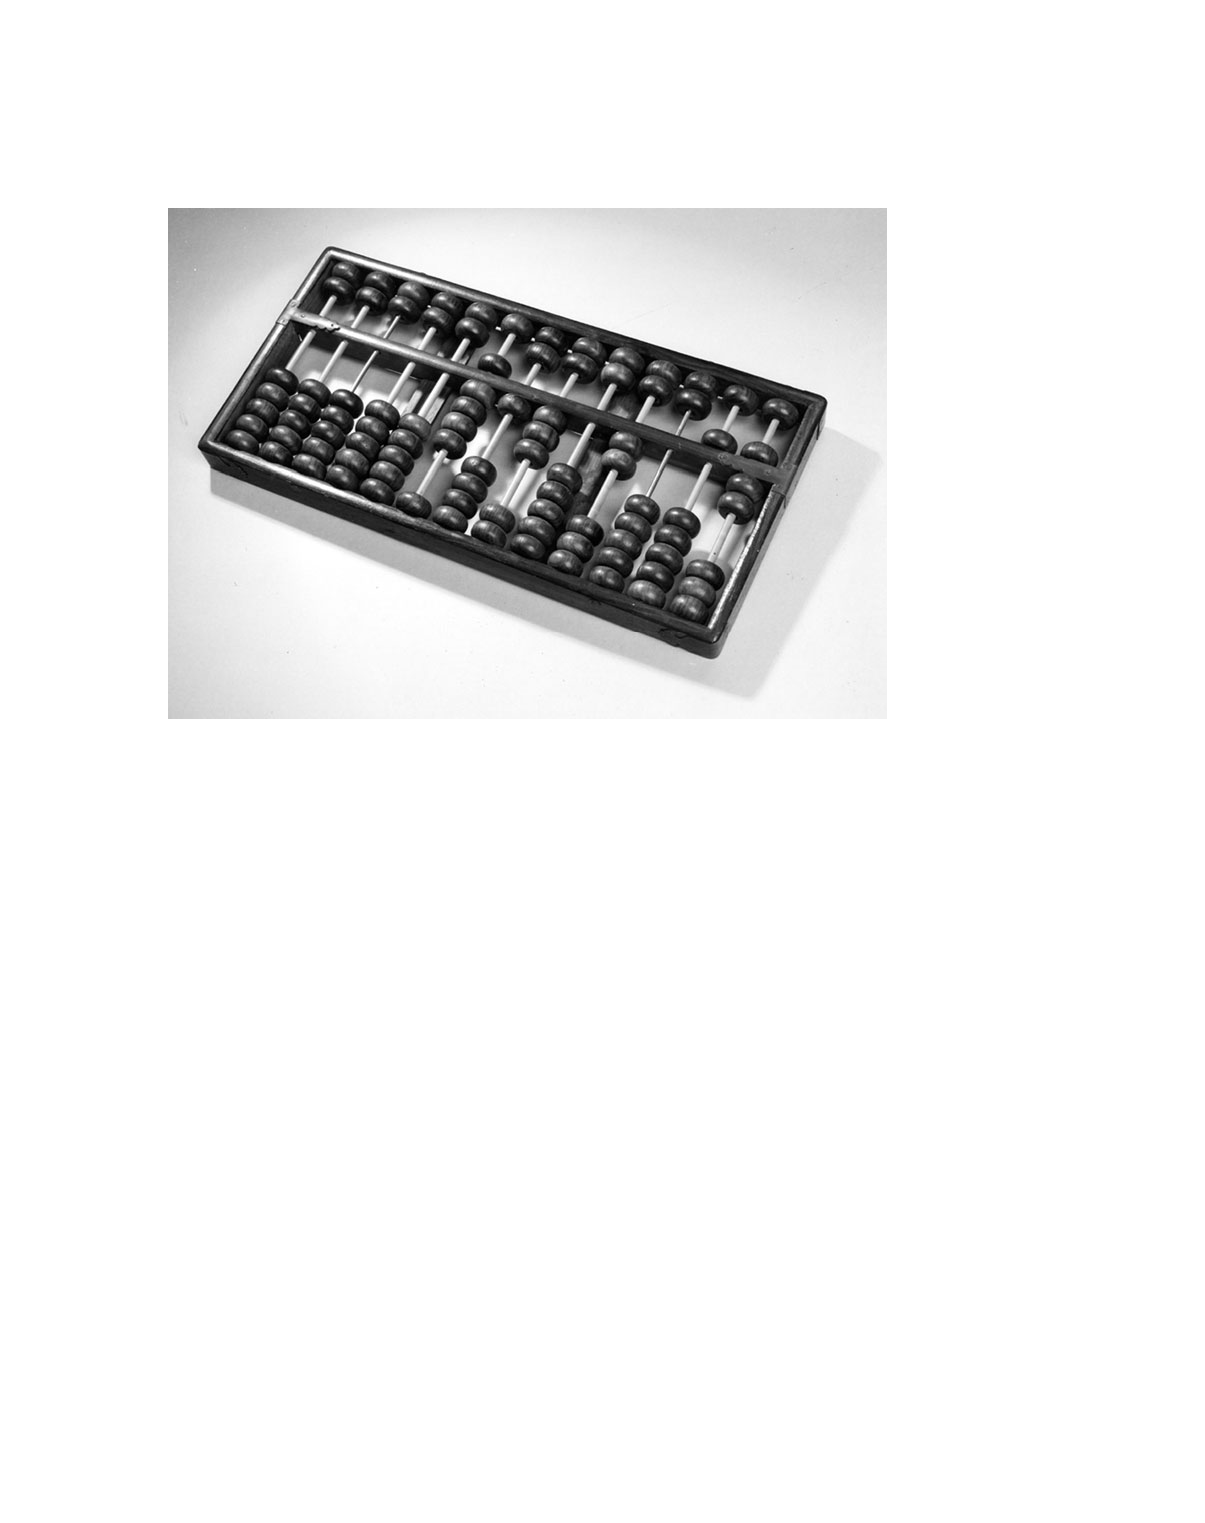
\includegraphics[width=4cm]{abaco.pdf}
\caption{Abaco}\label{fig:abaco}
\end{wrapfigure}
Il numero di simboli non può essere costante come nei sistemi posizionali, ma
deve crescere, cosa accadrebbe se vogliamo rappresentare $10^9$ in romano?
servono altri simboli dopo $\mathrm{M}$. Più importante ancora è la difficoltà
dell'aritmetica: Come possiamo descrivere le operazioni di somma o sottrazione?
In effetti tali operazioni non sono per nulla facili da descrivere, e
sicuramente sono decisamente più complesse rispetto all'aritmetica decimale. I
romani in pratica usavano fare le somme usando un \emph{abaco} (vedi Figura \ref{fig:abaco} accanto) 
solo per numeri molto piccoli.

Gli storici della matematica credono che l'uso della notazione posizionale decimale e l'introduzione dello \emph{zero} siano da attribuire a \emph{Brahmagupta} un matematico indiano nel 620\textrm{AD}. Questo sistema raggiunge l'Europa passando prima attraverso la Spagna (allora Musulmana) e diffondendosi in Italia. L'italiano Leonardo di Pisa, chiamato anche il Fibonacci, scopre questo sistema di numerazione e l'aritmetica ad esso associata lavorando nella bottega del padre, nella città di Bugia (una città Africana nella regione corrispondente all'attuale Algeria).
E' attraverso gli scritti di Muhammad ibn Musa al-Khwarizmi, Abu Kamil e altri\nota{Muhammad ibn Musa\\ al-Khwarizmi} matematici arabi che Fibonacci apprende il nuovo sistema, e lo diffonde in Europa dove viene presto adottato insieme all'uso dello zero. 

E' evidente\nota{Zero in\\ Matematica} l'importanza sia pratica (all'interno
del sistema di numerazione) sia concettuale dello zero. Il fatto che dovesse
esistere un \emph{numero} che indicasse un \emph{assenza} di quantità, è un
concetto che richiese secoli prima di essere assimilato. Lo zero è fondamentale
all'interno dei sistemi posizionali, lo studente oramai capisce la motivazione
di fondo: in un intero come $5005$, gli zeri sono essenziali per \emph{spostare
il peso di una cifra senza aggiungerne complessivamente al valore} (vedi i due
$5$). Una volta introdotto è necessario capire come le operazioni aritmetiche
si comportano su esso, e naturalmente si nota subito il problema legato alla
divisione. Il fatto che l'operazione di divisione \emph{non fosse definita}
(oggi diremmo che essa costituisce una funzione parziale sugli interi, vedi Appendice \ref{sec:fun}) è
qualcosa che contrariava molti matematici. Non parliamo delle resistenze dei
filosofi a dare un nome a una quantità per rappresentare....un assenza di
quantità.
}

\subsection{Conversione tra basi}\label{sec:conversione}

Di seguito si vedrà come convertire da una rappresentazione in base $b$ ad una
in base $B$. Poiché noi siamo abituati a svolgere operazioni in base $10$, per
facilitare il cambio di base, trasformeremo prima un valore dalla base $b$ di
partenza alla base $10$, e poi convertiremo il valore decimale ottenuto in base
$B$. Come visto anche nell'esempio $1$, la formula in \eqref{eq:pos} ci
consente di convertire un numero da una base qualunque alla base $10$. Pertanto
resta da capire come convertire da base $10$ ad un altra base generica $B$.
Osserviamo che dato un intero $n$, l'essenza della dimostrazione del Teorema
$1$ è la riscrittura dell'equazione \eqref{eq:pos} come\footnote{Questo è un
altro esempio del parallelismo tra numeri e polinomi, infatti questo modo di
scrivere i polinomi è detto formula di Horner ed è molto usata per velocizzare
la valutazione del polinomio in un punto.}:
\begin{align*}
n = \sum_{i=0}^{k-1} c_iB^i = (((c_{k-1}B+c_{k-2})B\ldots+ c_2)B + c_1)B + c_0\\
\text{i.e. } 1234 = ((1\cdot{10}+2)\cdot{10}+3)\cdot{10} + 4
\end{align*}

\noindent quindi la cifra meno significativa $c_0$ può essere ottenuta
dividendo (usiamo la divisione intera) $n$ per $B$ e prendendo il resto.
\nota{Conversione in base B, tramite divisioni ripetute per~B ed estrazione dei
resti.} Quindi abbiamo $c_0 = n \Mod{B}$ ed il valore della divisione $n' = n /
B$ è un intero formato dalle rimanenti cifre di $n$. Possiamo ripetere il
procedimento su $n'$ fin quando il valore della divisione è diverso da zero estraendo così tutte le cifre.

\begin{ex}
Consideriamo $n = 12345$, abbiamo $n' = n/10 = 1234$ e $n \Mod{10} = 5$. Ripetendo l'operazione di modulo su $n'$ otteniamo la cifra $4$, e così via. Se
invece di $10$ usiamo il valore della base $B$, otterremo valori tra $0$ e $B-1$, che non sono altro che le cifre di $n$ espresso in base $B$.

Convertiamo ad esempio $n = 12345$ in binario, scrivendo per ogni divisione il risultato della stessa $+$ il resto.

\begin{align*}
 12345 / 2 &= 6172 + 1   &96 / 2 = 48 + 0\\
 6172  / 2 &= 3086 + 0   &48 / 2 = 24 + 0\\
 3086  / 2 &= 1543 + 0   &24 / 2 = 12 + 0\\
 1543  / 2 &= 771 + 1    &12 / 2 = 6 + 0\\
 771   / 2 &= 385 + 1    &6 / 2  = 3 + 0\\
 385   / 2 &= 192 + 1    &3 / 2  = 1 + 1\\
 192   / 2 &= 96 + 0     &1 / 2  = 0 + \mathbf{1}& \quad \uparrow
\end{align*}

\noindent e poiché l'ultima cifra è la più significativa si ha che $12345$ in binario è $11000000111001$. Proviamo a convertire $58$ in esadecimale, osserviamo che $58/16 = 3$ e $58 \Mod{16} = 10$ quindi $(58)_{10} = (3A)_{16}$. Convertiamo $12345$ in ottale:
\begin{align*}
 12345 / 8 = 1543 + &1 \\
 1543  / 8 = 192 + &7   \\
 192  / 8  = 24 + &0 \\
 24  / 8   = 3 + &0
\end{align*}
\noindent Quindi $12345 = (30071)_8$.
\end{ex}

Il lettore è invitato adesso a confrontare la sequenza dei valori nei calcoli sopra con i valori ottenuti nella conversione in binario. Si nota facilmente che poiché $8 = 2^3$, ogni passo nella conversione in ottale, costituisce tre passi nella conversione decimale, è facile verificare che questo dipende direttamente dalle proprietà della rappresentazione in base. In ottale in effetti, ogni cifra è un valore tra $0$ e $7$, se vogliamo rappresentare questi valori in binario serviranno $\log 8$ bit, cioè $3$ bit per ogni cifra ottale.

Questo\nota{Conversione da binario ad ottale ad esadecimale} ci suggerisce un modo veloce per passare da una base $b$ ad una base $B=b^i$. Se si passa da $b$ a $B$ si tratta di \emph{raccogliere} ogni $i$ cifre e rappresentarle come un unica cifra in base $B$. Se viceversa si passa dalla base $B$ alla base $b$ allora ogni cifra si deve \emph{espandere} in $i$
cifre della base $b$.

\begin{ex}
Nell'esempio precedente $n=12345$ e in binario vale $11000000111001$, per passare velocemente in ottale, basta osservare che
\[
\underbrace{\mathbf{0}11}_{3}\underbrace{000}_{0}\underbrace{000}_{0}\underbrace{111}_{7}\underbrace{001}_{1}
\]
\noindent Notiamo che si inizia a raggruppare dalle cifre \emph{meno} significative, cioè da destra a sinistra, nel caso in cui come nell'esempio si hanno meno cifre di quelle da raggruppare, si devono aggiungere degli zeri, che posti a destra delle altre cifre (in figura in grassetto) non ne cambiamo il valore. Otteniamo
quindi esattamente il valore calcolato precedentemente. Lo stesso vale per la conversione in esadecimale, invece di usare le divisioni, poiché $16 = 2^4$ possiamo fare così:
\[
\underbrace{0011}_{3}\underbrace{0000}_{0}\underbrace{0011}_{3}\underbrace{1001}_{9}
\]
quindi $12345 = (3039)_{16}$, verifichiamolo: $3\cdot{16}^3+3\cdot{16}+1 = 12345$. Possiamo ovviamente fare lo stesso nella direzione contraria, cioè trasformare $(3039)_{16}$ in binario, espandendo le cifre esadecimali, nel corrispondente valore binario, basta \emph{girare} il senso delle parentesi graffe nello schema sopra, e cancellare i due zeri frontali (ridondanti).
\end{ex}

In Informatica l'uso della notazione ottale e sopratutto esadecimale consente
di rappresentare lunghe sequenze di bit in modo decisamente più compatto, un
numero binario di $32$ bit infatti richiederà solo $8 = 32/4$ cifre esadecimali.

Il metodo esposto sopra produce le cifre nell'ordine opposto rispetto al modo in cui noi scriviamo,  \nota{Conversione tramite divisioni per potenze decrescenti della base}
cioè da destra a sinistra, dalla meno alla più significativa. E' possibile ottenere la sequenza a partire da $c_{k-1}$ fino
a $c_0$, cioè nell'ordine in cui noi scriveremo il numero? Dalla \eqref{eq:pos},
abbiamo che per estrarre la cifra $c_{k-1}$ dobbiamo dividere il valore dell'intero che stiamo considerando, chiamiamolo $n$, per $B^{k-1}$. Ad esempio
se vogliamo estrarre $3$ da $3240$ dobbiamo dividerlo per $1000 = 10^3$, quindi dobbiamo sapere quante sono le cifre di $n$, ma questo si ottiene calcolando
$k = \lceil \log_{10} n \rceil$, notiamo che le restanti cifre sono contenute in $3240 \Mod{10^3} = 240$.

L'algoritmo pertanto è il seguente: Se si vuole convertire il numero decimale $n$ in base $B$ si calcola $k = \log_B n$, si calcola $c_{k-1} = n / B^{k-1}$ e $n' = n \Mod{B^{k-1}}$, si diminuisce $k$ e si applica lo stesso metodo a $n'$.

\begin{ex}
Convertiamo $3240$ in esadecimale usando il metodo sopra:
\begin{align*}
  &\lceil \log_{16} 3240 \rceil = 3\\
  3240 / 16^2 = 12 = &\, c_2, \qquad 3240 \Mod{16^2} = 168\\
  168 / 16^1 = 10 = &\, c_1,  \qquad 168 \Mod{16} = 8\\
  8 / 16^0 = 8 = &\, c_0.
\end{align*}
Quindi $3240$ in esadecimale è $\mathrm{CA}8$.
\end{ex}

\subsection{Aritmetica in base $B$}

L'aritmetica in base $B\neq 10$ segue esattamente le stesse regole di quella con i numeri decimali.

Cominciamo con l'operazione più semplice, il calcolo del successore di un intero $n$, valutare cioè $n+1$, questo ci consentirà di imparare a contare in una generica base $B$. Il lettore svolge questa operazione in modo \emph{meccanico} poiché l'ha appresa in tal modo fin dalle elementari.

Ma come possiamo formalizzare esattamente tale operazione?\nota{Contare in Base
$B$} E' facile verificare che il seguente Algoritmo è la risposta giusta:
esaminate le cifre del numero $n$ dalla meno significativa alla più
significativa fino a trovare la prima cifra minore di $B-1$ se esiste, cambiate
mentre si scorre verso sinistra ogni $B-1$ trovato in $0$. Se si trova una
cifra minore di $B-1$ si incrementa, altrimenti aggiungete una cifra pari ad
$1$ a destra del numero.

Lo studente provi a le seguenti operazioni in base $10$, seguendo l'algoritmo
espresso sopra: $139+1 = 140$, $99+1 = 100$. Notate inoltre che l'algoritmo presentato non è altro che l'algoritmo della somma imparato alle elementari ma presentato in modo leggermente diverso, senza usare i riporti per far scivolare
il valore del $+1$ verso sinistra. Lo stesso algoritmo si può quindi usare per contare in una base.
\nota{\vspace{1cm}Contare in basi diverse\\[1.5cm] Sommare in Binario}
\begin{ex}[Conteggio e Somma in base $B$]\label{ex:somma}
Contiamo in binario: $0, 1, (1+1) = 10$, $(10+1) = 11$, $(11+1) = 100$,
$100+1 = 101, 101+1 = 110$, etc.\\
Contiamo in base $3: 0,1,2,(2+1)=10,11,12,20,21,22,100$, etc.\\
Contiamo in base $4: 0,1,2,3, (3+1) = 10, 11,12,13,20,21,22,23,30$, etc.\\
Contiamo in base $8: 0,\ldots,7, (7+1)=10,11,12,13,14,15,16,17,20,\ldots$, etc.

Le operazioni aritmetiche quindi si svolgono in modo identico a quello imparato
alle elementari. Sommiamo $31+12$ in binario. Si ha: $31/2 = 15 + 1, 15/2 = 7 + 1, 7/2 = 3 + 1, 3 /2 = 1 + 1$, quindi $31 = (1111)_2$ con $12 = (8+4) = 1100_2$
\begin{align*}
    &1\qquad \qquad \leftarrow\text{resti}\\
	&1111+\\[-0.5ex]
	&1100\\[-2ex]
   \text{--}&\text{------}\\[-1.8ex]
   1&1011
\end{align*}
\end{ex}

che deriva dal fatto che: $1+0 = 1$, e $1+1 = 10$ quindi si riporta un resto
a destra, sopra ad esempio abbiamo segnato il resto riportato nella somma tra le cifre in seconda colonna. Nella prima colonna si ha quindi $1+1+1 = 11$ e quindi il risultato presenta una cifra in più.
Se il numero di cifre è limitato, ad esempio se nell'esempio sopra il numero di bit fosse limitato a $4$, il risultato sarebbe stato trocato a $1011$ ed il
bit scartato viene usato proprio per segnalare questa situazione chiamata \emph{errore di overflow} (trabocco)\nota{Overflow}.

La sottrazione tra due numeri $a,b$ con $a>b$ avviene come in decimale, nel caso in cui il sottraendo è maggiore del minuendo, avviene un prestito, tenendo conto del peso delle cifre: se prendiamo in prestito da sinistra un unità, diventano due unità (in generale $B$ unità) prestate a destra.\nota{Sottrazione in binario}

\begin{ex}[Sottrazione Binaria]
Calcoliamo $25-14$, abbiamo $25 = 11001$ e $14 = 1110$ quindi 
\[
\begin{matrix}
 4 & 3 &   2   & 1 & 0 & \text{indice colonna}\\
   & 2  & \underline{2} & 2 &   & \text{resti}\\[1ex]
\hline\\[-1ex]
 \underline{\mathsf 1} & \underline{\mathsf 1} & \mathsf 0  & \mathsf 0 & \mathsf 1 & \mathsf-\\
 \mathsf 0 & \mathsf 1 & \mathsf 1  & \mathsf 1 & \mathsf 0 & \\[-1ex]
\text{---}&\text{---}&\text{---}&\text{---}&\text{---}& \\[-1ex]
 \mathsf 0 & \mathsf 1 & \mathsf 0 & \mathsf 1 & \mathsf 1 &
\end{matrix}
\]
In effetti $(1011)_2 = 2^3+2+1 = 11 = 25-14$.
\end{ex}

Vediamo in dettaglio: nella colonna $0$ a destra abbiamo $1-0 = 1$,
nella colonna $1$ abbiamo $0-1$ e non possiamo farlo senza prestiti.
Quindi chiediamo in prestito dalla colonna $2$ che però è a zero, quindi proseguiamo e chiediamo un prestito dalla colonna $3$, dove abbiamo un $1$ (abbiamo evidenziato con una sottolineatura i valori da cui prendiamo in prestito).\nota{Sottrazione\\Regole sui Prestiti}
Il prestito della colonna $3$ diventa un due nella colonna $2$ (guardate la riga con i resti), da questo prediamo in prestito un unità, che diventa un $2$ nella colonna $1$.
A questo punto possiamo completare l'operazione in colonna 1, con $2-0-1 = 1$,
nella colonna $2$, abbiamo $0 - 1$ ma dobbiamo considerare un unità di resto rimasta e quindi otteniamo $1 - 1 = 0$. Nella colonna tre, abbiamo $0-1$ perché abbiamo preso in prestito, quindi nuovamente prendiamo in prestito dalla colonna $4$ ottenendo $2-1 = 1$, a questo punto la colonna quattro è $0-0=0$.
Il procedimento è complicato, sopratutto per la gestione dei resti, anche se in fondo si tratta dello stesso procedimento che usiamo con numeri decimali.

Se $a < b$, l'operazione (sui Naturali) di sottrazione non è definita e si verifica una situazione di \emph{errore di underflow}\nota{Underflow}.

La moltiplicazione segue le stesse regola usate per moltiplicare numeri
decimali, si vuol sottolineare qui solo un aspetto, di natura prettamente
\emph{computazionale}. Sappiamo che la moltiplicazione di $a \cdot b$ è
semplicemente la somma ripetuta di $a$ con se stesso per $b$ volte (e per la
proprietà di commutatività, anche la somma ripetuta di $b$ con se stesso $a$
volte). Come mai non usiamo questo procedimento per svolgere la
moltiplicazione?\nota{Moltiplicazione\\ Numero di Operazioni} (provate adesso a svolgere $145 \times 34$ senza calcolatrice).
Invece, come appreso alle elementari, moltiplichiamo $a$
\emph{per le singole cifre} di $b$ ($145 \times 3 = 435$, $145 \times 4 = 580$)
e scriviamo questi prodotti parziali incolonnandoli in modo relativo alla cifra corrispondente usata in $b$, poi sommiamo questi prodotti parziali ottenendo un valore ($435\times10+580 = 4930$).  Come mai questo valore corrisponde al prodotto? 

Lasciamo questo quesito al lettore (che probabilmente non si era mai posto tale
problema) qui invece sottolineamo che il motivo per cui svolgiamo la
moltiplicazione in questo modo è perche $\ldots\ldots$ \emph{è efficiente}.
Comporta cioè molte meno operazioni del metodo basato sulle somme ripetute,
dove per \emph{operazioni} intendiamo le somme e prodotti tra singole cifre: lo
studente provi a \emph{contarle} nei due casi.


\subsection{Numeri Interi Negativi}

Nella Sezione precedente, lo studente dovrebbe aver compreso come rappresentare
un numero naturale in una base arbitraria, come convertire tra basi diverse, ed
in particolare in binario, e nelle basi ad esso correlate (ottale,
esadecimale). Inoltre, dovrebbe saper contare in una qualunque base e svolgere
le operazioni di somma, sottrazione, moltiplicazione e divisione. Infine,
dovrebbe conoscere le relazioni che legano il valore di un numero rispetto al
numero di cifre che lo compongono nelle diverse basi.

In questa Sezione ci preoccuperemo di capire come rappresentare i numeri interi negativi, e quindi passare da $\mathbb{N}$ a $\mathbb{Z}$. Nell'uso comune i numeri negativi sono rappresentati aggiungendo un simbolo '$-$' davanti alla loro rappresentazione come numeri naturali positivi. Quindi abbiamo $1234$, e $-1234$, e questa è sicuramente la rappresentazione più semplice. Dal punto di vista astratto tale rappresentazione è perfettamente compatibile con la Definizione in \eqref{eq:pos}, infatti la applichiamo al sistema decimale senza problemi.

L'obiettivo di questa sezione è quindi leggermente più complesso: Non ci serve semplicemente una notazione per i numeri negativi, in base arbitraria, ma una notazione che li rappresenta senza usare simboli aggiuntivi rispetto all'insieme $\mathcal{C}$ definito in \eqref{eq:pos}. In altri termini: Poiché i computer memorizzano tutto in forma binaria, il sistema di rappresentazione che useremo per i numeri negativi deve essere compatibile con questa scelta, deve cioè consentire di \emph{codificare} interi positivi o negativi in modo che alla fine la rappresentazione del numero sia sempre e solo costituita da una stringa di bit. I sistemi di rappresentazione che vedremo, per quanto
definiti per basi arbitrarie, hanno una reale applicazione solo in binario.

\subsubsection{Modulo e Segno}

Il primo modo, molto semplice per codificare i numeri negativi è notare che i
simboli '$+$' e '$-$' per il segno, sono solo due, quindi possono essere
rappresentati usando un bit: associamo ad esempio $0 = $'$+$' e $1 = $'$-$', e
mettiamo questo bit davanti alla rappresentazione del valore assoluto del
numero.

\begin{defn}[Modulo e Segno] La rappresentazione \emph{con Modulo e
Segno} di un intero $n$ in binario con $k$ cifre è la seguente:
\[ n = (c_{k-1}c_{k-2}{\ldots}c_1c_0)_2 = (-c_{k-1}) \cdot \sum_{i=0}^{k-2}c_i2^i \]
\end{defn}

Notiamo quindi che il segno è rappresentato nella cifra più significativa che  non viene a far parte del \emph{valore} dell'intero come le altre cifre. Come si vede dagli indici della sommatoria il range di rappresentazione\nota{Numeri Interi in Modulo e Segno, con $k$ bit: Range = $[-2^{k-1}-1,2^{k-1}-1]$} è dato dagli interi nell'intervallo $[-2^{k-1}-1,2^{k-1}-1]$.

\begin{ex} Il valore $-12$ sarà ottenuto prima calcolando il valore del modulo
(valore assoluto) $12 = (1100)_2$ e poi aggiungendo un bit di segno messo ad
$1$, quindi $(-12 = 11100)$. Notiamo che abbiamo usato $5$ bit, infatti con
soli $4$ bit, dovendo usarne una per il segno, avremmo a disposizione solo $3$
bit per il valore assoluto, e quindi il massimo valore rappresentabile sarebbe
$111 = 7$. Con $5$ bit possiamo quindi rappresentare i valori interi in
$[-2^4-1,2^4-1] = [-15,15]$. In generale si deve sempre prestare attenzione a
fissare il numero di bit in modo che l'intervallo di rappresentazione sia
sufficientemente grande da poter rappresentare gli interi di nostro interesse.
\end{ex}

%% ----------------------- PYTHON TABLE ------------------
\begin{table}\sffamily
\renewcommand{\arraystretch}{1.2}
\begin{pycode}
print(r"\begin{tabular}{c|rccc}")
print(r"Binario & Posizionale & Modulo e Segno & Scostamento (a $7$) & Complemento a $2$ \\ \noalign{\smallskip}")
print(" \\hline\\noalign{\\smallskip}\n")
for i in range(16):
	print("%04s & $%2d$ & $%c%d$ & $%+2d$ & " % (format(i,'04b'), i , '+' if (i<8) else '-', i if (i<8) else (i-8), i-7),end=' ')
	print("$%+d$ \\\\ \n" % (i if (i<=2**3-1) else (-2**4+i)))
print("\hline\n \\end{tabular}")
\end{pycode}
\caption{Numeri binari di $4$ bit: valore rispetto alla notazione posizionale (naturali), e confronto dei valori nei vari sistemi per numeri negativi.}
\label{tab:zeta}
\end{table}

%% ----------------------- PYTHON TABLE ------------------


Nella Tabella \ref{tab:zeta} vediamo un confronto tra l'interpretazione di numeri binari con $4$ bit nei due sistemi visti finora. Notiamo che nella prima
colonna abbiamo aggiunto degli zeri davanti ad ogni numero in modo da
evidenziare sempre il numero di cifre che abbiamo fissato ($0000 = 0$). Come si
vede chiaramente ogni riga della tabella, nelle colonne dalla seconda in poi, presenta un modo diverso di \emph{interpretare} una certa sequenza di bit (della prima colonna). Quindi chiedersi quale sia il valore di una
certa sequenza di bit senza sapere quale sia il sistema di rappresentazione
usato è insensato.

Ad esempio nella prima colonna il valore della sequenza di bit $1010$
rappresenta il valore $10$ se si interpreta come un intero senza segno, se
invece la sequenza di bit rappresenta un valore scritto nella notazione con
modulo e segno allora essa vale $-2$. E' responsabilità di chi ha scritto la
sequenza di bit, sapere come interpretarla.

La rappresentazione in modulo e segno è semplice, ma presenta vari problemi che
hanno portato alla sua scomparsa nell'uso pratico. Notiamo dalla Tabella che
esiste sia il valore $+0$ che il valore $-0$, e questo comporta uno spreco
poiché due diverse sequenze di bit, sono di fatto associate allo stesso valore.
Inoltre la presenza di un bit di segno separato, rende più complicate le
operazioni aritmetiche di somma e sottrazione (ma facilita le
moltiplicazioni/divisioni). Vediamo un esempio di sottrazione:

\begin{ex} Proviamo a calcolare $25 - 14$: nel sistema con modulo e segno, per rappresentare $25$ serviranno almeno $6$ bit per la rappresentazione. Infatti $2^{6-1}-1 = 31 > 25$, mentre $2^{5-1}-1 = 15$ ed il valore $25$ non sarebbe rappresentabile con $5$ bit.

Abbiamo quindi $25 = 011001$ e  $-14 = 101110$. Adesso nasce un problema:
la sottrazione ha regole complicate sui prestiti, ma in algebra $a-b = a+ -b$ quindi proviamo a usare la somma tra $25$ e $-14$:
\begin{align*}
	    1&1 \quad \leftarrow\text{resti}\\
	    0&11001 \;+\\
	    1&01110\\[-0.5ex]
      &\text{--------}\\[-0.5ex]
	    ?&00111
\end{align*} L'operazione di somma, non si avvicina affatto
al risultato corretto: infatti $25-14=11$ su $6$ bit, con segno e modulo è rappresentato come $001011$. Quello che stiamo dicendo in pratica è che
il sistema di rappresentazione con modulo e segno non gode della proprietà: $a-b = (a)+(-b)$, che ci consentirebbe di trattare le sottrazioni come somme.
L'operazione di sottrazione andrebbe svolta come nell'Esempio 8, con le sue complicate regole sui prestiti.
\end{ex}

L'osservazione\nota{Modulo e Segno\\ problemi con l'ALU} sopra va intesa alla luce, di quello che vedremo nel Capitolo successivo sull'ALU, cioè sul circuito che internamente al Processore svolge le
operazioni aritmetiche. Se adottassimo la notazione con modulo e segno, dovremmo avere una parte circuitale che confronta i segni, per controllare se
sono discordi/concordi, e due circuiti diversi, per la somma e per la sottrazione da usare nei due casi. Come vedremo esistono
rappresentazioni che possiedono la proprietà algebrica $a-b = (a)+(-b)$,
quindi necessitano in hardware solo di un circuito per la somma. Ecco
uno dei motivi principali per cui la notazione con modulo e segno non è usata all'interno del calcolatore.

\subsubsection{Rappresentazione in Scostamento}\label{sec:offset}

Un altro modo di rappresentare i numeri negativi è la rappresentazione in scostamento (offset) rispetto ad un valore. Si usa una semplice traslazione
per consentire di associare a numeri negativi, una rappresentazione che normalmente sarebbe associata ad un valore positivo.

Il ragionamento per definire questa rappresentazione è molto semplice. I valori
rappresentabili con $k$ cifre in base $B$ tramite \eqref{eq:pos} sono gli interi in $[0,B^k-1]$. 

\begin{defn}
Sia $M > 0$ intero, la rappresentazione \emph{in Scostamento ad $M$} di un intero $n$ con $k$ cifre è la seguente:
\[  n = (c_{k-1}\,\cdots\,c_{0})_B = \sum_{i=0}^{k-1} c_iB^i - M \]
\end{defn}

\noindent allora il range di rappresentazione sarà: $[-M,B^k-M-1]$. Di solito
si considera $M = B^k/2-1$ se vogliamo circa metà di valori positivi e metà
negativi. Il range dei valori rappresentati andrà dal minimo $-B^k/2+1$ fino al
massimo $B^k-1-(B^k/2-1) = B^k/2$ per $B=2$ si ha l'intervallo:\nota{Rappresentazione in Scostamento\\ Intervallo di Rappresentazione\\in Binario:\\ $[-2^{k-1}-1,2^{k-1}]$}
$[-2^{k-1}-1,2^{k-1}]$. Ad esempio, con $k = 8$ bit, abbiamo i valori tra
$[-2^7+1,2^7] = [-127,128]$. Nella Tabella \ref{tab:zeta} vediamo un esempio con $4$
bit, e range $= [-7,8]$. Notiamo che il bit più significativo resta associato
al segno ma con il significato opposto al caso precedente, se il numero è
negativo il bit è a \emph{zero}, positivo se vale uno, e lo zero sotto questa
interpretazione è un \emph{meno zero} poichè $0 = 0111$ ed il bit alto vale
zero. Notiamo anche che i numeri positivi non conservano la loro
rappresentazione rispetto alla notazione senza segno, e questo è una debolezza
di questo sistema.\medskip

\begin{ex} I numeri decimali con al massimo $2$ cifre vanno da $0$ a $99$. In decimale con scostamento a $M = -10^2/2 + 1 = -49$ otteniamo gli interi nell'intervallo $[-49,50]$. Il simbolo $\mathsf 0$ deve quindi essere interpretato come $0-49 = -49$, e allo stesso modo si ha: $\mathsf{1} = -48$, $\mathsf{49} = 49 - 49 = 0$ e $\mathsf{99} = 99 - 49 = 50$.

In Binario con otto bit e scostamento $M = 127$ abbiamo i valori interi nell'intervallo: $[-127,128]$. Se prendiamo quindi un numero $11011011$, il suo valore si ottiene convertendolo in decimale:
$11011011 = 219$ e sottraendo $127$ quindi si ha $(11011011) = 92$. Viceversa se avessimo dovuto \emph{codificare} il valore di $92$, avremmo prima calcolato $92+127$ e successivamente convertito tale valore in binario.
\end{ex}\medskip

Questo tipo di rappresentazione è usata non tanto per rappresentare i valori interi (negativi o positivi), ma per un uso più specifico: rappresentare l'esponente\nota{Esponente in IEEE-754} nella notazione in standard \textrm{IEEE-754} per i numeri in virgola mobile, come vedremo nella sezione a loro dedicata.

\subsubsection{Rappresentazione in Complemento alla Base}


La rappresentazione \emph{in Complemento} è l'ultima che presenteremo ed è da molti anni, quella realmente utilizzata all'interno del calcolatore per
rappresentare tutti gli interi. Illustriamo subito le proprietà
di cui essa gode, rispetto alle altre rappresentazioni viste finora:
\begin{enumerate}
	\item Rispetta la proprietà algebrica:  $a - b = a +\, -b$. Quindi le sottrazioni, possono essere svolte come semplici somme.
	\item Come nel modulo e segno, il bit più alto individua il segno del numero, zero se positivo, uno se negativo. Quindi un test come $a > 0$ o $a < 0$
	richiede il controllo del valore di un singolo bit.
	\item I numeri positivi sono associati alla stessa sequenza di bit della notazione dell'equazione \eqref{eq:pos}. Quindi la parte positiva della
	codifica corrisponde perfettamente a quanto visto per i naturali (vedi Tabella \ref{tab:zeta}).
\end{enumerate}

La rappresentazione in complemento alla base sfrutta una proprietà fondamentale
di ogni sistema numerico \emph{con un numero finito di cifre}. Se infatti usiamo al massimo $k$ cifre, (abbiamo ripetuto oramai numerose volte che) il massimo valore rappresentabile è $B^k-1$. Notiamo quindi che il valore
$B^k$ \emph{non è rappresentabile}. In particolare cosa accade se calcoliamo $B^k-1\,+\,1$ avendo solo $k$ cifre?

\begin{ex} In decimale con tre cifre abbiamo:
	\[ \boxed{9}\boxed{9}\boxed{9} + 1 = 1\;\boxed{0}\boxed{0}\boxed{0} \]
E poiché l'uno a sinistra non può essere scritto, abbiamo $10^3 = 1000 \equiv 0$. Lo studente di matematica attento ha già capito che in pratica la somma lavora \emph{modulo $1000$}. Ad esempio: con tre cifre decimali, il valore di $-45$ è $55$, perché se calcoliamo $45 + 55$ si ha $100 \equiv 0$.
\end{ex}

Consideriamo quindi l'anello $Z_{B^k}$ e le sue classi di resto. Ad esempio la
classe $[1] = 1 + (B^k)\mathbb{Z}$ indica tutti gli interi che sono congrui ad
uno modulo $B^k$, e cosi via. Tipicamente si usano come rappresentanti le classi $[0] \ldots [B^k-1]$, ma questo è solo una scelta, che può
essere cambiata. In particolare, se vogliamo lavorare con valori negativi
possiamo scegliere come rappresentanti i valori da $[-B^{k-1}]$ a $[B^{k-1}-1]$.

\begin{wrapfigure}[9]{r}{4cm}\vspace{-3ex}
 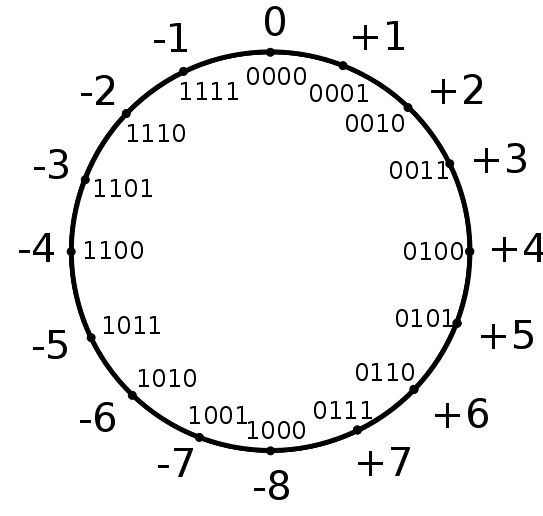
\includegraphics[width=4cm]{2Komplement.png}
 \label{fig:comp2}
\end{wrapfigure}

\begin{defn}[Complemento alla Base]
Dato $n \in \mathbb{N}$, e fissato il numero di cifre della rappresentazione $k$, definiamo \emph{complemento alla base} l'intero $n'$ che soddisfa $n'= B^k-n$.
\end{defn}
\noindent ad esempio in decimale con due cifre, il complemento a
$dieci$ di $45$ è $55 = 100-45$. Nella Tabella \ref{tab:zeta} vediamo un
esempio di rappresentazione con $4$ bit, in \emph{complemento a due}, e nella figura accanto, osserviamo l'interpretazione modulare del sistema.\nota{Complemento a Due}

Osserviamo facilmente che questo sistema soddisfa le proprietà elencate nei
punti sopra: Il bit più significativo è zero se il numero è
positivo, uno se negativo (punto 2); Il complemento a due di $5 = 0101$ ad
esempio è $16-5 = 11 = 1011 = -5$, come si vede in tabella. Vale quindi che
$0101+1011 = 0$ (punto $1$). Inoltre, i valori positivi sono rappresentati dalle stesse stringhe di bit usate per rappresentare i naturali (i numeri positivi nella quinta colonna sono uguali a quelli della seconda)
quindi vale il punto $3$.

Possiamo adesso definire il valore di una sequenza di cifre in complemento alla base come:

\begin{defn}[Complemento alla Base]
La rappresentazione \emph{in Complemento alla Base} di un intero $n$ 
con $k$ cifre è la seguente:
	\[ n = (c_{k-1}c_{k-2}{\ldots}c_1c_0)_2 = (-c_{k-1}B^{k-1}) + \sum_{i=0}^{k-2}c_iB^i \]
\end{defn}

Mostriamo inoltre come calcolare il complemento alla base senza effettuare
esplicitamente la sottrazione $B^k - n$. Poichè siamo particolarmente
interessati al sistema binario, lavoriamo con $B=2$.  
Il complemento a due di $n$ è $2^k - n$ che scriviamo come $2^k-1-n+1$. Definiamo \emph{complemento ad uno}\nota{Complemento ad Uno} il valore $m = 2^k-1-n$. In generale avremo un \emph{complemento alla base $-1$} definito come $m = B^k-1-n$ ed il complemento alla base è uguale a $m+1$. 
Adesso notiamo che il complemento alla base $-1$ è facilmente calcolabile
senza svolgere sottrazioni, poichè il valore di $B^k-1$ è sempre costituito in ogni base da una sequenza di $k-1$ cifre tutte uguali a $B-1$, esse sono quindi sempre maggiori di ogni cifra in $n$ e la sottrazione nel calcolo del complemento ad uno, può essere fatta senza considerare prestiti e analizzando solo una cifra alla volta. In binario questo corrisponde all'operazione di \emph{complemento} o \emph{not} dei bit, dove \textsf{not} $0 = 1$, e \textsf{not} $1 = 0$. Gli
esempi chiariranno meglio il significato di quanto detto:

\begin{ex} Calcoliamo il complemento a due di $45$ ($-45$).

\noindent \textbf{Primo metodo:} Prima di tutto per rappresentare $45$ in
questo sistema dobbiamo avere almeno $7$ bit, infatti con $6$ bit il massimo
valore rappresentabile è $2^{6-1}-1 = 31 < 45$, con $7$ abbiamo $2^6-1 =
63>45$. A questo punto sappiamo che $-45 = 2^7-45 = 83$ e $83$ in binario è
$1010011$ (usando uno dei metodi in \ref{sec:conversione}).\medskip

\noindent \textbf{Secondo Metodo:} Questo metodo non userà sottrazioni, ed è
quello usato davvero in hardware dai circuiti dell'ALU. Sappiamo che servono
$7$ bit, abbiamo $45 = 32+8+4+1 = 101101$, quindi $0101101$. Adesso notiamo che
il complemento ad uno di $45$ è dato da $2^7-1-45$, e $2^7-1 = 127 = 1111111$.
Calcoliamo $1111111-0101101$, notiamo che in ogni passo $1-1=0$ e $1-0=1$
quindi la sottrazione corrisponde all'operazione di \emph{complementazione
binaria}, o \emph{negazione bit-a-bit}, in cui ogni $0$ diventa $1$ e ogni $1$
diventa $0$. Quindi il complemento ad $1$ di $45$ è $1010010$ (notiamo che è
essenziale sapere su quanti bit si sta lavorando e aggiungere sempre gli zeri
di fronte, prima di complementare). A questo punto il complemento a due è
$1010010+1 = 1010011 = 83$. \end{ex}

Mostriamo adesso alcune operazioni di somma con addendi di segno diverso e le
loro particolarità: 

\begin{ex}
Calcoliamo $50 - 36$, e $36 - 50$, le operazioni sono presentate nella sequente tabella, con la riga dei resti sopra gli addendi. 
\begin{center}\vspace{-1cm}
\begin{minipage}[t]{0.4\textwidth}
	\begin{align*}
50-36:\\
	\mathsf{_1}&\mathsf{_{1\; 1\, 1\; \;\;\; 1\; 1\; 1}}\\
		   &00110010\;+\\
		   &11011011\\[-1ex]
	       &\text{------------}\\[-1ex]
		  1&00001110
	\end{align*}
\end{minipage}
\hspace{1cm}
\begin{minipage}[t]{0.4\textwidth}
\begin{align*}
36-50:\\
       &\mathsf{_{\quad\;\;\; 1\, 1\;\; 1\, 1}}\\
	   &00100100\;+\\
	   &11001101\\[-1ex]
       &\text{------------}\\[-1ex]
	   &11110010
\end{align*}
\end{minipage}
\end{center}

Cominciamo con l'operazione a sinistra: $50$ in binario è $110010$, su $6$ bit
senza segno. Ma lavorando in complemento a due, quel valore sarebbe negativo
(bit alto ad uno), quindi \emph{dobbiamo sempre, fissare il numero di cifre con
cui lavoriamo}, ad esempio usiamo $8$ bit (un byte). Quindi abbiamo $50_{10} =
00110010$ (bit alto a zero, correttamente poichè $50 > 0$).

Adesso calcoliamo il complemento a due di $36$: il modulo è $32+4 = 00100100$,
complementiamo tutti i bit, $11011011$, e la somma da il risultato
corretto è $00001110 = 14 > 0$, con un bit di overflow da trascurare (non segnala una condizione di errore). Notiamo che abbiamo usato
il complemento ad uno come operando, ma abbiamo anche messo ad $1$ il resto sulla prima cifra, trasformando quindi il complemento ad uno, nel complemento
a due, come parte dello svolgimento dell'addizione.
Nella parte destra , vediamo come svolgere l'operazione invertendo
gli operandi, quindi $36-50$. Il secondo operando è il complemento ad uno di
$50$ come nel primo caso, ed il risultato è correttamente $-14$ in complemento a due.
Nel caso in cui i valori sono dello stesso segno, l'operazione si svolge allo stesso modo, ma può capitare che il risultato sia fuori dal range di rappresentazione (maggiore di $127$ o minore di $-128$), questo è segnalato
dal bit di overflow che sarà di segno diverso rispetto al segno degli operandi.
\end{ex}


\textbf{Riassumendo}: 
Lo studente adesso conosce tre modi diversi per rappresentare
valori negativi: la rappresentazione in modulo e segno, in scostamento, ed in
complemento alla base. Egli deve essere in grado di convertire un intero decimale in una qualunque di queste rappresentazioni specialmente nel caso
binario, ed in particolare per il sistema in complemento a due.
Deve anche conoscere gli intervalli di rappresentazione in funzione del numero di bit disponibili. 

\section{Numeri Razionali e Reali}

La sezione precedente ha trattato i numeri Naturali e gli Interi, adesso
vediamo come rappresentare numeri non interi, quindi in $\mathbb{Q}$ o
$\mathbb{R}$. Notiamo che i valori di $\mathbb{Q}$ potrebbero essere
rappresentati come coppie di interi $p, q$ con $mcd(p,q) = 1$. Questa notazione
presenta alcuni vantaggi: il valore della frazione è rappresentato senza
perdere informazioni (senza errori di approssimazione), ma le operazioni
aritmetiche sono complesse. Naturalmente questa notazione non sarebbe
utilizzabile per $\mathbb{R}$. Preferiamo quindi trattare in modo uniforme gli
elementi di $\mathbb{Q}$ e $\mathbb{R}$, parleremo in generale della
rappresentazione di un numero reale, sapendo che se è un intero esso ricade in
quanto descritto nelle sezioni precedenti altrimenti la sua rappresentazione è
basata su una semplice estensione del Teorema 1:
\begin{thm}
\label{thm:F}
Sia $B>1$ la base del sistema di rappresentazione, $\mathcal{C}$ un insieme
di $B$ cifre distinte, allora $\forall\, x \in \mathbb{R}$, l'espansione in base $B$ di $x$ è una sequenza (infinita) di cifre $c_{k-1}c_{k-2}{\cdots}c_0\mathbf{.}c_{-1}c_{-2}\cdots$ con $c_i \in \{0,...,B-1\}$ tali che:
\begin{equation}\label{eq:reali}
	x = \sum_{i=0}^{k-1} c_iB^i + \sum_{i=1}^{\infty} c_{-i}B^{-i}
\end{equation}
\end{thm}

Nella \eqref{eq:reali} abbiamo una prima sommatoria che corrisponde alla parte
intera di $x$, e la seconda che corrisponde alla parte frazionaria. Le cifre
vengono scritte a destra di un punto che separa le potenze della base positive
da quelle negative: es. $234.345 =
(2\cdot10^2+3\cdot10+4)+(3\cdot10^{-1}+4\cdot10^{-2}+5\cdot10^{-2})$. Le cifre
della parte frazionaria possono essere infinite poiché se $x$ è un razionale
periodico o un irrazionale, la sua espansione decimale non è finita. Inoltre
l'unicità è garantita solo se imponiamo delle equivalenze come $0.999999\ldots = 1$\footnote{Il lettore può trovare interessante, a questo punto, rivedere la definizione di numero reale studiata nel corso di Analisi I}.

All'interno del calcolatore useremo una rappresentazione con un numero finito
di cifre (bit)\nota{Errore di Troncamento}, quindi dovremo in generale fissare la lunghezza della parte
frazionaria e se necessario \emph{troncare} il vero valore di $x$. Questo
introduce un \emph{errore di troncamento} o di \emph{rappresentazione}
inevitabile; lo studio di come tali errori influenzino le operazioni che
usano questi numeri porta alla nascita del \emph{Calcolo
Numerico}.

Riguardo alla conversione tra basi diverse, abbiamo trattato la gestione della
parte intera nella sezione precedente, prima di entrare nel dettaglio della
rappresentazione interna al calcolatore mostriamo come convertire in
particolare da decimale a binario la parte frazionaria.
Usando lo stesso ragionamento fatto per la parte intera, dobbiamo
\emph{estrarre} il valore delle cifre frazionarie, da $c_{-1}$ in poi. 
Notiamo che \[
B(x - \left\lfloor x \right \rfloor) = c_{-1} + \sum_{i=2}^{\infty} c_{-i}B^{-i+1}
\implies c_1 = \left\lfloor B(x - \left\lfloor x \right\rfloor) \right\rfloor \]
e le altre cifre possono essere estratte allo stesso modo.\nota{Metodo della Moltiplicazioni per la Base} 
Quindi se per estrarre le cifre della parte intera usavamo un metodo basato
sulle divisioni ripetute per la base, in questo caso usiamo un metodo basato
su \emph{moltiplicazioni} ripetute per la base.
Vediamo un esempio, prima in decimale, e poi di conversione da decimale a binario.

\begin{ex} Usiamo $x = 3.78125$. La parte frazionaria è $x-\left\lfloor x \right \rfloor = 0.78125$, adesso
$0.78125\cdot 10 = 7.8125$ e $\lfloor 7.8125 \rfloor = 7$. 
Adesso ripetiamo con la parte frazionaria $0.8125$, \emph{moltiplicando} per la base estraiamo le cifre da sinistra verso destra.
Se invece di moltiplicare per $10$, usiamo la base in cui vogliamo scrivere le
cifre, ad esempio in binario otteniamo:
\begin{align*}
		 0.78125 \cdot 2 &= 1.56250\\
		 (1.56250-1) \cdot 2 &= 1.125\\
		 0.125 \cdot 2 &= 0.25\\
		 0.25  \cdot 2 &= 0.5\\
		 0.5 \cdot 2 &= 1.0
\end{align*}
quindi prendendo le parti intere si ha: $(.78125)_{10} = (.11001)_2$, verifichiamolo: $1/2+1/4+1/32 = 0.5 + 0.25 + 0.03125 = 0.78125$. Notiamo che se fissiamo a $5$ il numero di bit della parte frazionaria, il numero immediatamente più grande di $.11001$ è $.11010 = 1/2 + 1/4 + 1/16 = 0.8125$, quindi ogni numero reale $x$ con $0.78125  < x < 0.8125$ non può essere rappresentato esattamente, ma dovrà essere approssimato.

Notiamo che il procedimento sopra può generare una sequenza infinita di bit, che dovrà essere necessariamente troncata, ad esempio proviamo a convertire
in binario $17/5 = 3.4$ usando $3$ bit per la parte intera e $5$ bit
per la parte frazionaria: la parte intera è $3_{10} = 011_{2}$, la parte frazionaria $0.4$ in binario sarà:
\begin{align*}
		 0.4 \cdot 2 &= 0.8\\
		 0.8 \cdot 2 &= 1.6\\
		 0.6 \cdot 2 &= 1.2\\
		 0.2 \cdot 2 &= \mathbf{0.4}
\end{align*}
notiamo che dopo $4$ moltiplicazioni otteniamo di nuovo il valore iniziale $0.4$; da questo momento in poi è evidente che si ripeterà la sequenza di cifre $0110$ continuamente. Pertanto il valore esatto per la parte frazionaria sarebbe $\overline{0110}$. La rappresentazione troncata è $011.01101 = 3.40625$.
con un \emph{errore assoluto} pari a $3.4 - 3.40625 = 0.00625$ e relativo di $0.00625/3.4 \approx 1/1000$ (che segnala l'errore nella terza cifra della parte frazionaria).
\end{ex}

\subsection{Aritmetica in Virgola Fissa}

La rappresentazione vista nella sezione precedente, costruita a partire dal Teorema $2$ fissando a priori il numero di cifre
per la parte intera, e per la parte frazionaria è detta \emph{rappresentazione in virgola fissa}. 

Il motivo per cui si usa tale dizione nasce da una semplice osservazione: una volta fissato il numero complessivo di cifre del sistema, ad esempio $t$ cifre, ed il valore di $k$ (il numero di cifre della parte intera), la parte frazionaria avrà $f = t-k$ cifre, ed il punto rimarrà
sempre fisso tra le prime $k$ e le rimanenti $f$ cifre. 

Notiamo che anche se dal punto di vista teorico, i sistemi\footnote{Uso il plurale perche fissato $t$ abbiamo vari sistemi al variare di $k$.} in virgola fissa servano a rappresentare numeri frazionari, essi in pratica \emph{manipolano interi}. Non è necessario memorizzare il valore di $k$ o di $f$: dato $n \in \mathbb{N}$ con $n \leq B^t-1$ esso rappresenterà il razionale $x = n / B^f$: ogni numero quindi viene memorizzato come un intero e considerato implicitamente diviso per $B^f$,  $f$ è detto anche \emph{precisione} della rappresentazione.
Ad esempio, se $t = 8$, e $k = 3$, il valore di $x = 345.67814$ verrà rappresentanto con l'intero $34567814$. In binario, questo significa che possiamo usare i numeri interi, rappresentati magari in complemento a due,
per rappresentare numeri in virgola fissa. Di solito la dimensione $t$ è
un multiplo di $8$, la dimensione esatta dipende da come è stata costruita l'ALU, quindi è essenzialmente legata al tipo di processore. Nei processori
moderni, l'ALU può manipolare numeri interi di $32$ o $64$ bit ($4$ o $8$ byte)
pertanto, il valore di $t$ è uno tra essi, il programmatore sceglie di solito il valore di $f$ a seconda della precisione necessaria nei calcoli, e da questo deriva poi il range dei valori rappresentabili. 

Questo sistema di rappresentazione è molto comodo se il processore non possiede unità dedicate per lavorare con numeri frazionari, ed era molto usata negli anni $'70$ ed $'80$ anche se presenta vari problemi che illustreremo immediatamente. Nei calcolatori moderni è stata rimpiazzata dallo standard IEEE 754 che usa una rappresentazione in \emph{virgola mobile} (\emph{floating-point}), tale rappresentazione è più efficiente nell'uso delle cifre, migliorando quindi la precisione dei calcoli, inoltre essa si presta facilmente ad essere implementata tramite un circuito dedicato, detto FPU (\emph{floating-point unit} l'analogo dell'ALU per i calcoli non interi).
La\nota{MIPS\\ FLOPS}, velocità di questi due circuiti, misurata in \textsc{MIPS}: \textbf{M}illion of \textbf{I}nteger operation \textbf{P}er \textbf{S}econd, e \textsc{FLOPS}: \textbf{FL}oat \textbf{O}peration \textbf{P}er \textbf{S}econd, sono stati per molto tempo indicatori molto diffusi delle \emph{performance} di un calcolatore, nell'ambito scientifico, dove si usano più frequentemente dati in virgola mobile, si guarda ancora oggi al numero di Giga\footnote{Giga = $10^9$, Tera = $10^{12}$, sono prefissi standard (sistema internazionale) per indicare i multipli di un unità di misura, come lo studente dovrebbe sapere dal corso di Fisica I} $Flops$ o Tera $Flops$ di un calcolatore.  Vediamo adesso il problema principale legato alla rappresentazione in virgola fissa. Calcoliamo questi valori in decimale, il risultato infatti è simile cambiando la base.

Fissiamo i valori di $t, k, f$, ad esempio $t = 8$, $k = 5$ e $f = 3$, il range dei valori rappresentabili nel caso di valori senza segno è il seguente: Il minimo è zero ed il valore massimo è dato da $99999.999$, quindi avremo $10^5 - 1$ per la parte intera e $0.999 = 1-0.001 = 1 - 10^{-3} = 1-10^{-f}$, quindi il massimo valore è $10^k-10^{-f} = 100000 - 0.001 = 99999.999$.
Supponiamo di voler rappresentare un numero intero come $100001$, nonostante
questo valore abbia solo $6$ cifre, esso non è rappresentabile nel sistema sopra poichè la suddivisione tra parte intera e parte frazionaria è \emph{rigida}, lo stesso vale per $0.323423$, nonostante abbia solo $6$ cifre esso non può essere rappresentato, infatti useremo una cifra nella parte intera per lo zero, e le $4$ cifre restanti saranno sprecate, costringendoci a troncare la parte frazionaria a $3$ cifre. La conclusione ovvia è che nei sistemi di rappresentazione in virgola fissa, lo spazio (le cifre) non sono usate in modo efficiente.

\subsection{Numeri Floating-Point - IEEE 754}

I problemi della rappresentazione in virgola fissa hanno portato allo sviluppo
della notazione in virgola mobile che è probabilmente già conosciuta dallo
studente come \emph{rappresentazione in notazione scientifica}. Partendo dai
problemi della notazione in virgola fissa, l'idea che vogliamo realizzare è la
sequente: fissiamo il numero di cifre complessivo ($t$), vogliamo
poter mettere la virgola dove ci pare (\emph{floating}) in modo da poter
usare le $t$ cifre per la parte intera se serve, o per la parte frazionaria, a seconda del valore da rappresentare. 

Per far questo, notiamo che se ho $x = 45.346$ posso
spostare la virgola \emph{lasciando invariato} il valore di $x$ se e solo se
tengo conto di tale spostamento, moltiplicando o dividendo $x$ per una potenza
opportuna della base: \[ 45.346 = 4.5346\cdot{10^1} = 0.45346\cdot{10^2} =
453.46\cdot 10^{-1} = 45346\cdot 10^{-3}\]
ed in generale abbiamo un infinità di modi per scrivere $x$. Recuperiamo
l'unicità se decidiamo tra tutte le rappresentazioni di usare quella con
l'esponente che porta un unica cifra \emph{diversa da zero} a sinistra del
punto e le restanti tutte a destra, tale scelta viene detta
\emph{normalizzazione} del valore di $x$. Nel caso sopra useremo $x =
4.5346\cdot{10^1}$. Vale pertanto il seguente Teorema di rappresentazione:

\begin{thm}[Notazione in virgola mobile]
\medskip
Dato un numero reale $x \in \mathbb{R} \neq 0$, ed una base $B>1$ esistono:
 \begin{itemize}
	 \item un segno $s = \text{sign}(x)$,
	 \item un unico valore $m = c_0.c_{-1}c_{-2}\ldots$ chiamato \emph{mantissa}, formata da una sequenza (eventualmente infinita) di cifre con $0 \leq c_i < B$, e $c_0 \neq 0$,      \item un esponente $e \in \mathbb{Z}$.
 \end{itemize} per cui vale:
\[ x = (-1)^s m B^e = (-1)^s \cdot c_0 + \left(\sum_{i=-1}^{\infty} c_iB^{-i} \right)\cdot B^e \]
\end{thm}

Il Teorema sopra può essere usato per definire un insieme \emph{finito} di valori, detti \emph{numeri di macchina} ed indicati con $\mathbb{F}(B,n,t,q)$ dove $n$ è il numero complessivo di cifre usate, $t$ è il numero di cifre usate per la mantissa e $q$ il numero di cifre per l'esponente. Notiamo che lo zero non fa parte di questo insieme.

Lo standard \textsc{IEEE-754}\nota{Sistema IEEE-754} usato nei computer moderni estende $\mathbb{F}(B,n,t,q)$ con lo zero (rappresentato in modo particolare), ed altri valori, tra cui: un insieme di numeri \emph{de-normalizzati} (con $c_0 = 0$) e alcuni speciali come $\pm \infty$ ed un \emph{non-valore} detto \emph{Nan} (Not a Number) la cui utilità verrà spiegata successivamente. 

Vediamo intanto la rappresentazione  di un numero in \text{IEEE-754}:
prima di tutto fissiamo la base, vi sono processori che lavorano in base $10$, ma la base prevalente è quella binaria; il numero complessivo di cifre può variare tra tre dimensioni: $n = 32$ bit o \emph{singola precisione}, $64$ bit o \emph{doppia precisione} e in alcuni casi \emph{quadrupla precisione} $128$ bit. 

Il segno ($s$) è sempre rappresentato tramite il bit più significativo (quindi la notazione è simile alla modulo e segno), subito dopo viene rappresentato l'esponente. Quest'ultimo è un valore con segno, e lo si scrive con una rappresentazione con scostamento (vedi Sezione \ref{sec:offset}). Infine vi sono i bit che rappresentano la mantissa, che si rappresentano con una particolarità: nel caso di numeri normalizzati, poichè $c_0 \neq 0$, allora si ha $c_0 = 1$ (perche siamo in base $2$). La cifra $c_0$ essendo costante, non è memorizzata esplicitamente, quindi la mantissa contiene le rimanenti cifre $c_{-1}....c_{-t}$.

Dato il segno $s$, la mantissa $m$ e l'esponente $e$, il valore rappresentato (per i numeri normalizzati) è: 
\begin{equation}\label{eq:normalnumber} 
	x = (-1)^s\, (1+m)\, 2^{e-\text{bias}} 
\end{equation}

Sotto vediamo il formato IEEE-754 nel caso di numeri in singola o doppia precisione.\bigskip

\mdfdefinestyle{mdf}{leftmargin=3cm,rightmargin=2cm,%
  innerleftmargin=1cm,innerrightmargin=1cm,roundcorner=10pt,backgroundcolor=green!10}
\begin{mdframed}[style=mdf]
\footnotesize
\hspace{4.5cm}\begin{tabular}{llc}
	1 bit & 8 bits    & \hspace{1cm}23 bits\\[-1ex]
	segno & esponente & \hspace{1cm}mantissa\\
\end{tabular}
\vspace{-2ex}\small\flushright
$\qquad \boxed{0}\boxed{010\ldots\ldots 100}\boxed{10101010101 \ldots 10101010101}$\\
$\qquad _{31}\;_{30}\quad\ldots\qquad _{23}\;_{22} \qquad \ldots\qquad\qquad\qquad\qquad\;_0$
\begin{center}\sffamily IEEE-754 - Singola Precisione - 32 bits \end{center}
\footnotesize\flushleft\hspace{0.2cm}
\begin{tabular}{llc}
	1 bit & \hspace{0.6cm}11 bits    & \hspace{2cm}52 bits\\[-1ex]
	segno & \hspace{0.6cm}esponente & \hspace{2cm}mantissa\\
\end{tabular}
\small\flushright
$\qquad \boxed{0}\boxed{010\ldots\ldots\ldots\ldots 100}\boxed{10101010101 \text{\hspace{1.2cm}}\ldots\ldots\ldots\text{\hspace{1.2cm}} 10101010101}$\\
$\qquad _{63}\;_{62}\qquad\quad\ldots\qquad\quad _{52}\;_{51} \text{\hspace{3.2cm}}\qquad \ldots\qquad\qquad\qquad\qquad\;_0$
\begin{center}\sffamily IEEE-754 - Doppia Precisione - 64 bits \end{center}
\end{mdframed}

\begin{ex}
	Convertire $-5.828125$ in IEEE-754 in singola precisione:
	
	Cominciamo con la parte intera: $5 = 4+1 = (101)_2$, (potevamo usare anche il metodo della divisione ripetuta per $2$). Per la parte frazionaria abbiamo, seguendo il metodo delle moltiplicazioni per la base: $0.828125 \times 2 = 1.65625$, quindi la prima cifra è $1$, poi ripetiamo su $0.65625$ e cosi via, fino ad ottenere $1101010$. Quindi abbiamo $5.828125_{10} = 1.011101010\times 2^2$ normalizzato. 
	
	L'esponente va codificato in scostamento a $2^7-1=127$, quindi: $2+127 = 129$ e in binario $129 = 128+1 = 10000001$ infine il segno è negativo quindi in definitiva abbiamo
	\[ -5.828125 = 1\;10000001\;01110101000000000000000 \]
in esadecimale più compattamente 0xC0BA8000 (il prefisso '0x' è un altra notazione per indicare che il numero adiacente è in base $16$).
\end{ex}
Poichè l'esponente è di $8$ bit, il range di valori va da $0$ a $255$. I valori estremi sono usati per rappresentare valori particolari, come vedremo tra poco, mentre i valori validi per l'esponente dei numeri normalizzati varia da $1$ a $254$, e corrisponde al range di esponenti validi $-126 \ldots 127$.
I valori (positivi e negativi) più vicini allo zero sono pertanto $1.0 \times 2^{-126} \approx \pm 1.17549 \times 10^{-38}$ mentre il valore più lontano da zero è fatto da una mantissa di tutti $1$ ed esponente pari a $127$ quindi: 

\[ 2^{127} \sum_{i=0}^{23} 2^{-i} =  2^{104} \sum_{i=0}^{23} 2^i = 2^{104}\, (2^{24}-1) \approx 3.4028 \times 10^{38} \]

Abbiamo visto che se l'esponente vale $0$ o $255$, i valori rappresentati sono particolari:
\begin{itemize}
	\item Lo zero non è un numero normalizzato ($c_0 = 0$) e viene rappresentato con tutti i bit a zero. Notiamo che come nella rappresentazione
	con mantissa e segno, esiste un $+0 = 0x00000000$ ed un $-0 = 0x80000000$ a seconda del valore del bit del segno.
	\item Quando l'esponente è posto con tutti i bit ad uno, e se la mantissa è tutta a zero, questo non rappresenta come dovrebbe $\pm 1.0 \times 2^{126}$ ma
	rappresenta a seconda del valore del bit di segno due valori speciali $\pm \infty$. 
	\item Se l'esponente è sempre con tutti i bit ad uno, i.e. $126 (+127)$ ma la mantissa è diversa da zero, allora abbiamo un particolare valore detto \textsc{NaN} $=$ \emph{Not a Number} per indicare il risultato di operazioni non definite: $1/0$ o $\sqrt{-1}$.
\end{itemize}

Resta la sola possibilità ancora non considerata di un esponente a zero e di una
mantissa diversa da zero. Questi numeri sono chiamati \emph{denormalizzati} e
in pratica corrispondono alla stessa espressione dell'Equazione \ref{eq:normalnumber} ma con il bit implicito $c_0 = 0$ e non $c_0 = 1$ (quindi non $(1 + m)$ ma semplicemente $m$). Questi numeri, sono chiaramente più piccoli dei numeri normalizzati o meglio più vicini allo zero, e servono esattamente a ridurre l'errore in quell'intervallo.

Per lo studente di matematica la comprensione delle limitazioni legate alla
rappresentazione con numeri floating-point è molto importante. Per approfondire
ulteriormente al di là di queste note, un riferimento interessante è il
seguente: \href{http://www.validlab.com/goldberg/paper.pdf}{"What Every Scientist Should Known About Floating-Point Arithmetic"} (scaricabile 
cliccando sul nome dell'articolo) o all'indirizzo: \url{http://www.validlab.com/goldberg/paper.pdf}.

Abbiamo concluso la parte legata alla rappresentazione in binario di numeri interi, naturali e con segno, e di numeri non interi, frazionari, e reali (approssimati tramite numeri floating-point a precisione limitata). Nella prossima sezione vedremo come si rappresentano le informazioni di tipo non numerico.

\section{Testi, Immagini, Musica}

Come sappiamo, i calcolatori moderni possono manipolare oltre che numeri, anche informazioni più complesse: testi, in varie lingue, immagini fisse in bianco e nero e a colori, video e audio. In questa sezione vedremo come è possibile trasformare queste informazione in forma binaria.

In tutti i casi, le rappresentazioni verranno costruite tramite \emph{codifiche}
che trasformano quelle informazioni di cui sopra in sequenze di numeri interi.
Dal punto di vista matematica vedremo che queste codifiche degli \emph{isomorfismi}, molto semplici da applicare. 

\subsubsection{Testi}
 Cominciamo con l'informazione non-numerica di tipo più seplice,\emph{un testo}. I testi, formalmente sono \emph{stringhe}, cioè sequenze finite di caratteri, dove i possibili caratteri sono presi da un insieme finito detto \emph{alfabeto}. Anche questo testo che leggete soddisfa questa definizione,
 in quanto, possiamo vederlo come una lunghissima sequenza di caratteri (dell'alfabeto Italiano, unito a tutti i caratteri di interpunzione e allo spazio). Poichè l'insieme di simboli dell'alfabeto è per ipotesi \emph{finito},
 possiamo associare ad ogni simbolo un numero intero positivo, ad esempio potremmo definire: \textsf{A}$=65$, \textsf{B}$=66 \ldots$ \textsf{Z}$=132$, etc; come mai non ho associato \textsf{A}$=1$, etc; dal punto di vista teorico
qualunque biezione tra i simboli dell'alfabeto ed un opportuno sottoinsieme di $\mathbb{N}$ andrebbe benissimo, ma quella fatta sopra è un estratto di una codifica standard, per i testi, chiamata \emph{Codifica ASCII}. Il lettore può consultare Internet per avere la tabella completa (ad esempio cercando la voce \texttt{ASCII} su Wikipedia), e troverà le corrispondenze tra ogni possibile simbolo della tastiera di un calcolatore, compresi quelli non stampabili come lo spazio e il \emph{ritorno carrello}, e molti altri.

Quindi un testo è una sequenza di caratteri codificati come interi, tramite il codice ASCII, quest'ultimo associa ad ogni carattere un byte (otto bit). Notiamo che, poichè un byte sono otto bit, il numero massimo di caratteri diversi che possiamo rappresentare in ASCII sono esattamente $256$. L'ASCII è stato per tanto tempo la sola codifica standard, ma nell'ultimo decennio esso è stato superato da codifiche più complesse come UTF-8/Unicode. Non entreremo nel dettaglio di questi aspetti, noi consideremo nel corso di Programmazione  i testi come semplici sequenze di interi (ottenuti tramite la tabella ASCII).

\subsubsection{Musica}

Un suono formalmente è \emph{un'onda} rappresentabile come una
funzione contina del tempo, descritta da opportuni parametri come l'ampiezza, la
frequenza, etc. E' abbastanza chiaro al lettore, vista la sua formazione matematica, e quanto detto finora, che una funzione \emph{continua} non potrà mai essere rappresentata esattamente all'interno di un calcolatore. Innanzitutto il suono deve avere lunghezza
finita, ad esempio $t$ secondi. Possiamo trasformare il segnale audio in modo che esso sia descrivibile da una funzione continua $Sound: T \mapsto D$, dove $T
= [0,t]$ è il tempo, e $D = [-A,A]$ con $A \in \mathbb{R}$ è l'ampiezza massima
del segnale.

A questo punto dobbiamo attraversare due fasi di \emph{discretizzazione} per trasformare il dominio e il codominio da insiemi \emph{continui} a \emph{discreti} (ed in particolare \emph{finiti}). La discretizzazione del dominio (il tempo) si chiama nello specifico \emph{campionamento del segnale}, e consiste nella forma più semplice nel 
decidere i punti in cui valutiamo la funzione $Sound$, a passi regolari, ad esempio $M$ valutazioni nell'intervallo $[0,1]$ ($M$ campioni/secondo). 
Esiste un Teorema (di Nyquist) che dice che se la frequenza di campionamento è il doppio della massima frequenza presente in $Sound$, allora se campioniamo con frequenza maggiore o uguale a questo valore, il segnale discreto così ottenuto può essere \emph{interpolato} per ricostruire senza perdita il segnale originale.

Ad esempio, l'udito umano è sensibile alle frequenze fino a $22kHz$, pertanto se campioniamo con una frequenza di $44kHz$ un segnale audio, (quindi se raccogliamo circa $44000$ campioni al secondo) otteniamo un segnale \emph{discreto} che però contiene in un certo senso tutta l'informazione del segnale continuo originario. Ecco perche se notate l'etichetta di un CD-Audio, troverete che il segnale è campinato esattamente a $44.1 kHz$.

\begin{wrapfigure}[14]{r}{5cm}
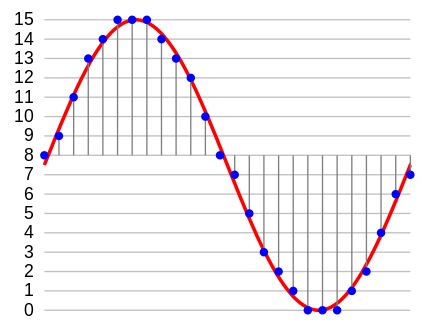
\includegraphics[width=5cm]{Pcm.png}
\caption{\footnotesize Campionamento e Quantizzazione di un Segnale Continuo ad una dimensione (Audio)}
\end{wrapfigure}

Nella Figura accanto la fase di campionamento corrisponde a valutare la
funzione nei punti indicati. Adesso dobbiamo discretizzare il codominio, e
questa fase si chiama \emph{quantizzazione}, infatti il valore della funzione è
una quantità continua nel codominio $[-A,A]$ e come tale non rappresentabile
senza errori. La quantizzazione, decide quanti bit usare per rappresentare un
valore del codominio, ad esempio se usiamo $16$ bit, abbiamo $2^{16} = 65536$
il valore $0$ corrisponderà a $-A$, il valore $65535$ a $A$, con i valori su
una griglia di passo $1/65536$. A questo punto, possiamo memorizzare i $44100$
campioni per secondo (frequenza di campionamento di $44.1$ kHz, dove per ogni
campione useremo due byte ($16$ bit). In questo modo, se prendiamo una canzone
di lunghezza media (circa $3$ minuti e mezzo) abbiamo $3.5\times60 = 210s$ per
ogni secondo usiamo $2*44100$ byte, per un totale di $18522000$, cioè $
18522000 / (1024\times 1024) = 17.66$ MB (MegaByte). Normalmente noi
memorizziamo queste informazioni in forma compressa (ad esempio tramite i
formati con perdita \textsf{.mp3} o senza perdita \textsf{.flac}), impiegando
una frazione minore di spazio.

Come si vede, anche in questo caso, abbiamo trasformato un informazione di tipo
non numerico in una sequenza di interi.

\subsubsection{Immagini, Video}

Il procedimento impiegato per codificare la musica, può essere usato allo stesso
modo con segnali bidimensionali come le immagini. In questo caso, la funzione a due variabili $Img(x,y): [0,MAXX]\times[0,MAXY] \mapsto Colors$ associa ad ogni punto del piano, un valore che rappresenta il colore del segnale visivo in quel punto. Il procedimento di campionamento, consiste nel determinare una \emph{griglia} di dimensione finita, e valutare la funzione nei punti della griglia. Il numero complessivo di punti verrà chiamato \emph{risoluzione} dell'immagine, ed ogni punto viene chiamato \emph{pixel}. La fase di quantizzazione, consiste nel decidere come il colore di un punto viene rappresentato: se usiamo una \emph{sintesi additiva} il colore sarà la somma di alcune frequenze primarie, ad esempio, la somma di una certa quantità di Rosso, di verde (Green) e di Blue, determina un sistema chiamato \textsf{RGB}. Se
per specificare queste quantità si usa, un byte per ognuna, otteniamo un totale di $256 \times 256 \times 256 \approx 16M$ sfumature possibili.

Ad esempio, una immagine catturata con uno smartphone con una fotocamera digitarle di $10$Mpixel, occuperà $4$ byte (si preferisce dedicare un numero di byte pari ad ogni punto, quindi ad i $3$ byte per il rosso, verde, e blu, se ne aggiunge un altro non usato) per pixel, per un totale non compresso di $10 \times 1024 \times 1024 \times 4 \approx 41$MB. Se confrontate questo numero con la dimensione media di un immagine compressa in formato \textsf{.jpg} (in media circa $1$MB) capite quanto siano efficaci gli algoritmi di compressione usati.

Quindi, se una canzone dentro il vostro calcolatore è rappresentata da una sequenza di interi, una immagine sarà una \emph{matrice} di (quadruple) di interi.

\chapter{Architettura del Calcolatore}

In questo Capitolo vedremo come è strutturato un Computer moderno.

\textbf{da completare}

%!TEX root = note.tex

\chapter{Introduzione}

\section{Algoritmo: Etimologia e Significato}

La nozione di \textbf{Algoritmo} è la nozione centrale dell'Informatica, la sua piena comprensione è fondamentale per l'attività di scrittura di programmi al calcolatore.

Secondo Knuth \cite{knuth} La parola Algoritmo deriva da \emph{Muhammad ibn Musa \'l-Khwarizmi}, un matematico persiano che scrisse nell'anno 825 un famoso libro sulle regole per il calcolo delle operazioni aritmetiche, come somma, sottrazione, moltiplicazione e divisione tra numeri in notazione araba (la notazione decimale usata adesso comunemente).

Il termine algoritmo deriva dall'errata associazione tra i procedimenti descritti nel libro ed il nome dell'autore. I matematici moderni usano questo termine per denotare dei procedimenti di calcolo che terminano in tempo finito con un risultato e descritti in modo rigoroso, passo per passo. Intorno al 1950 la parola algoritmo è frequentemente associata all'algoritmo di Euclide. 

\section{Un Idea Intuitiva di Algoritmo}

Esistono moltissimi formalismi atti ad esprimere algoritmi, tra cui:
\begin{itemize}
 \item La \emph{Macchina di Turing} è sotto molti aspetti, il più importante modello di calcolo. Esso fornisce la 
  definizione moderna del concetto di Algoritmo (Turing, 1936).
 \item Funzioni $\mu$-ricorsive, un formalismo basato sulle funzioni e sulla loro composizione definito da Church and Kleene (1936).
 \item Il $\lambda$-calcolo, un formalismo algebrico basato sul concetto di funzioni $\mu$-ricorsive, usato
 attualmente come notazione per la descrizione della semantica dei linguaggi funzionali, presentato
 sempre da Church nel 1936. Turing dimostra l'equivalenza tra $\lambda$-calcolo e le sue macchine
 nel 1937.
 \item Grammatiche a struttura di frase. Un sistema di riscrittura di termini, usate adesso per descrivere la sintassi dei linguaggi di programmazione. E' stato dimostrato anch'esso Turing equivalente.
 \item Tanti altri, tra cui: RAM (Random Access Machine), Algoritmi di Markov, Modelli di Post, e ovviamente ogni moderno linguaggio di programmazione.
\end{itemize}

Ognuno di questi formalismi, cerca di catturare in modo diverso la nozione di Algoritmo.
Indipendentemente dal formalismo usato un algoritmo deve soddisfare i seguenti requisiti, descritti informalmente:

\begin{itemize}
\item Un algoritmo è costituito da un insieme finito di istruzioni;
\item Ogni istruzione appartiene ad un insieme finito di istruzioni possibili, questo insieme è chiamato generalmente \emph{set d'istruzioni}. Ogni istruzione ha un effetto limitato su dati discreti, scegliere un opportuno set d'istruzioni corrisponde a   descrivere un \emph{modello di calcolo} (o Macchina Virtuale);
\item La computazione è eseguita per passi discreti (singoli), senza ricorrere a sistemi analogici o metodi continui;
\item Nel caso in cui ogni passo dipenda solo dai precedenti e da una porzione finita dei dati, in modo deterministico (cioè: senza essere soggetti ad alcuna distribuzione probabilistica non banale), l'algoritmo si dirà \emph{Deterministico}; Se invece, l'ordine dei passi dipende da un generatore di numeri pseudo-casuale\footnote{Un generatore pseudo-casuale è un algoritmo \emph{deterministico} che genera una sequenza di valori, che \emph{appare} casuale. Nel senso che essa risulta difficilmente distinguibile da una sequenza estratta ad esempio da una variabile aleatoria continua uniforme su $[0,1]$}  allora l'algoritmo si dirà \emph{Probabilistico}.
\item Non c’è limite al numero di passi necessari all’esecuzione di un algoritmo, nè alla memoria richiesta per contenere i dati (finiti) iniziali, intermedi ed eventualmente finali.
\end{itemize}

Sotto queste ipotesi, tutte le formulazioni fin ad ora sviluppate sono equivalenti e si postula che lo saranno anche tutte le future (\emph{Tesi di Church-Turing}).


%\chapter{Linguaggi di Programmazione}
\section{Linguaggi di Programmazione}

Si è sempre sostenuto che la nostra capacità di ragionare è ciò che ci distingue dalle altre specie: sembrerebbe paradossale a prima vista tentare di meccanizzare ciò che è più specificatamente umano. Eppure queste note iniziano con una breve storia dei tentativi di \emph{meccanizzazione} del ragionamento umano, un processo che ha avuto un enorme sviluppo a partire dagli inizi del secolo scorso.

Perfino gli antichi greci sapevano che il ragionamento è un processo strutturato e che, almeno parzialmente, è governato da leggi esplicitabili. Aristotele codificò i sillogismi, Euclide la geometria; intorno alla metà del secolo scorso, i logici inglesi George Boole, e Augustus De Morgan andarono molto più avanti di Aristotele nel codificare le forme di ragionamento strettamente deduttivo. Tutti questi sforzi erano diretti a chiarire cosa si dovesse intendere esattamente con il termine di \emph{dimostrazione}.

In ogni caso, per poter ragionare e comunicare i loro risultati in modo preciso necessitavano di un particolare linguaggio, un \emph{sistema formale}. Esempi di sistemi formali sono il \emph{calcolo dei predicati} o gli enunciati della \emph{logica del primo ordine}, ed i \emph{linguaggi di programmazione}. Questi ultimi sono dei linguaggi artificiali, usati per descrivere \emph{algoritmi}, ovvero procedimenti risolutivi di problemi, atti ad
essere eseguiti da un calcolatore.

Un programma non è altro che la traduzione (si dice anche implementazione) di un algoritmo in uno specifico linguaggio
di programmazione. I linguaggi di programmazione, così come altri linguaggi coinvolgono due aspetti che è importante distinguere: la \emph{sintassi} e la \emph{semantica}. La sintassi ha a che fare con la \emph{struttura} (o la forma) dei programmi esprimibili in un dato linguaggio. La semantica, invece, ha a che fare con il \emph{significato} dei programmi esprimibili in un dato linguaggio.

Se consideriamo i linguaggi naturali, per esempio l'italiano, due frasi come ''\emph{la mela mangia il bambino}'' e ''\emph{il bambino mangia la mela}'' obbediscono entrambe alla sintassi dell'italiano (sono corrette sia ortograficamente che grammaticalmente), d'altra parte solo la seconda ha un significato, o semantica, ragionevole. Queste note iniziano con una definizione formale di questi concetti: Cominceremo con il termine \emph{linguaggio} come sinonimo di \emph{insieme di frasi (sintatticamente) ammissibili}. In altri termini: una volta fissato un\emph{alfabeto} $\Sigma$ di elementi base detti sinboli \emph{terminali}, un linguaggio non sarà altro che un sottoinsieme di tutte le frasi ottenibili come sequenze di simboli terminali. Tali sequenze saranno anche riferite con il termine di \emph{stringhe} (o parole) su $\Sigma$.

Si pensi ad esempio al linguaggio delle espressioni dell'aritmetica, ottenibili a partire dai numeri interi e dalle quattro operazioni $+, -, /, \times$. Fra tutte le possibili stringhe di numeri ed operazioni, ve ne sono di ammissibili\footnote{Nei linguaggi formali una stringa ammissibile è detta anche \emph{formula ben formata (fbf)}} come $3 \times 4+2$ e di non ammissibili come $3+\times+4$.

Quindi, il linguaggio delle espressioni aritmetiche può essere identificato come il sottoinsieme delle stringhe ammissibili. In modo del tutto analogo, un linguaggio di programmazione può essere identificato con l'insieme delle proprie stringhe ammissibili, che chiameremo comunemente \emph{programmi}. Descrivere la sintassi di un linguaggio significa quindi descrivere l'insieme delle stringhe del linguaggio, ovvero avere un metodo per:

\begin{itemize}
\item decidere quali stringhe fanno parte di tale insieme, e quali no, oppure
\item costruire tale insieme, enumerando le stringhe che lo compongono.
\end{itemize}

Il problema è quindi: come identifichiamo le stringhe ammissibili, che caratterizzano un linguaggio?
Esistono due approcci principali: Il primo si basa su uno strumento detto \emph{automa} che è in grado di
\emph{riconoscere} (o accettare) tutte e sole le stringhe che fanno parte del linguaggio.  Il secondo, si basa su un altro formalismo detto \emph{grammatiche}, che sono invece in grado di \emph{generare} (o costruire) tutte e sole le stringhe che fanno parte di un linguaggio. La teoria che studia questi aspetti è conosciuta come ''teoria degli automi'' o ''teoria dei linguaggi formali'', queste note introducono rapidamente questi due strumenti, senza scendere nei dettagli della teoria, al fine di comprendere i metodi con cui si descrive la sintassi dei linguaggi di programmazione.


%\chapter{Introduzione}

\section{Concetti}

\subsection{Esempio: l'Algoritmo di Euclide}

Problema: Dati due interi $m,n$ trovare il massimo comune divisore
(mcd).

\begin{enumerate}
\item (dividi) Calcola $m$ diviso $n$, sia $r$ il resto della divisione ($0 \leq r < n$).
\item (test zero). Se $r = 0$ allora termina con $mcd = n$.
\item (scambio). $m \leftarrow n$, $n \leftarrow r$ e ritorna al passo 1.
\end{enumerate}


\begin{ex}
Eseguite i passi del procedimento descritto per $n=2166$,
$m=6099$.\end{ex}

\begin{ex} Scrivere un algoritmo per la soluzione di equazioni di
secondo grado, descrivendo i passi con una notazione simile a quella
usata per l'algoritmo di Euclide.\end{ex}


Notiamo alcune caratteristiche importanti della descrizione di questo procedimento:
\begin{itemize}
\item I passi del procedimento sono ordinati in modo da non generare
  alcuna ambiguità sull'ordine delle operazioni. I passi sono eseguiti
  a partire dal primo in sequenza a meno di indicazioni esplicite
  contenute nelle istruzioni stesse (passo 3).
\item L'operazione $\leftarrow$ è detta \textbf{operatore di
    assegnamento}, la sintassi $m \leftarrow n$ significa che il
  valore della variabile $n$ sostituisce il valore associato alla
  variabile $m$.
\item L'operazione $m = n$ è il classico test equazionale di
  eguaglianza matematica ($m$ è uguale ad $n$?). La differenza
  rispetto all'operatore $\leftarrow$ è enorme. L'eguaglianza valuta
  espressioni e confronta valori, ma non cambia il contenuto delle
  variabili (cambiamenti di stato). L'operatore di assegnamento invece
  descrive un azione da compiere, un cambiamento dello stato,
  attraverso la variazione del contenuto di una variabile.
\item Ad esempio se $n \in \mathbb{N}$, $n = n + 1$ è matematicamente
  sempre falso, mentre l'operazione $n \leftarrow n + 1$ indica
  semplicemente l'incremento del valore associato alla variabile $n$.
\end{itemize}

\section{Algoritmi e Linguaggi}

La notazione usata nell'Algoritmo di Euclide include:
\begin{itemize}
 \item variabili e costanti.
 \item l'operatore di assegnamento ($\leftarrow$)
 \item operatori di uguaglianza ($=$), possiamo aggiungere,
   facilmente, anche ($\neq, <, >, \leq, \geq$).
 \item Istruzioni condizionali: (se \verb|<condizione>| allora
   \verb|<comando>|)
 \item Istruzioni di salto: (\verb|vai a <numero>|,
   \verb|ritorna a <numero>|).
 \item Possiamo aggiungere per comodità un altra notazione per
   indicare un insieme di variabili indicizzate con un
   intero,comunemente usate in matematica per denotare valori con un
   pedice: $x_1,\ldots,x_n$. Tale notazione viene modificata
   generalmente in $x[1],\ldots,x[n]$.
\end{itemize}

Questo tipo di notazione è detta anche \emph{pseudo-linguaggio}, e viene usata per scrivere algoritmi. La notazione può essere arricchita ulteriormente ma permette già così di esprimere ogni possibile algoritmo (cosa significa questo con precisione verrà chiarito successivamente).

A partire dal modello matematico possiamo definire con precisione dei problemi.  Dato un problema, lo studente dovrà trovare l'algoritmo di risoluzione, cioè la sequenza di passi (scritti con la notazione dello pseudo-codice) che a partire dai dati iniziali costruiscono una soluzione del problema. Una volta trovato un Algoritmo corretto per la risoluzione di un problema, un Programma è una rappresentazione in un linguaggio di programmazione dell'Algoritmo.

Notiamo quindi che la differenza sostanziale tra il concetto di Algoritmo e quello di Programma, riguarda solamente il linguaggio con cui essi sono espressi.  Nel primo caso, lo pseudo-linguaggio consente un astrazione maggiore ed ha come scopo, lo studio delle proprietà formali (terminazione, correttezza) dell'algoritmo. Nel secondo, invece, i linguaggi di programmazione sono costruiti per facilitare al calcolatore la fase di esecuzione.

Il significato moderno del termine algoritmo assomiglia a quello di una ricetta, metodo, tecnica, procedura, routine per svolgere un compito (calcolare dei valori). Ma la nozione di algoritmo è molto di più. Non tutte le sequenza finite di operazioni specificano un algoritmo.

\subsection{Algoritmi: Caratteristiche}

\begin{description}
\item[Finitezza] Un algoritmo è descritto da un numero finito di passi (finitezza sintattica).  L'algoritmo di Euclide inoltre è \emph{corretto} poichè se la sequenza di passi termina, allora stampa sempre il valore corretto del mcd. Inoltre è possibile dimostrare che esso termina sempre.
\item[Non Ambiguità (Definiteness)] Ogni passo dell'algoritmo è completamente definito, per evitare ambiguità si usa una notazione matematica con sintassi e semantica non ambigue come lo pseudo-codice, non si usa il linguaggio naturale (come l'italiano). Nell'algoritmo di Euclide questo significa che esiste un agente di calcolo (lo studente, o il calcolatore) che interpreta esattamente le operazioni di divisione intera, calcolo del resto, test di eguaglianza con $0$, etc.
\item[Input] Ogni algoritmo riceve zero o più valori di input dall'esterno, i valori di input dell'algoritmo di Euclide sono ad esempio valori interi. Nota: per essere ancora più precisi, nell'algoritmo di Euclide dovrebbe essere incluso un passo $0$ con un istruzione del tipo: $m \leftarrow \mbox{ input }, n \leftarrow \mbox{ input }$. Dove input è una variabile speciale che contiene tutti i valori passati in input al problema in sequenza.
\item[Output] Un algoritmo restituisce un output, un risultato del problema. L'algoritmo di Euclide restituisce il massimo comune divisore tra m,n. Infatti dopo il passo 1, si ha $m = qn+r$ con $q \geq 0$. Se $r = 0$, allora $m$ è un multiplo di $n$ e $mcd = n$. Altrimenti se un numero divide $m,n$ deve dividere anche $m-qn = r$, inoltre ogni numero che divide $n,r$ divide $qn+r=m$. Quindi l'insieme dei divisori comuni di $m, n$ coincide con l'insieme dei divisori di $n, r$ (e quindi anche il massimo dei divisori è lo stesso). Da qui la validità del passo 3.
\end{description}

\subsection{Algoritmi: Effettività}
Questo è il punto più importante tra le caratteristiche della nozione di algoritmo.

Ogni operazione svolta in un algoritmo deve essere effettiva. Questo significa che essa deve essere sufficientemente semplice da poter essere eseguita (in principio con carta e penna) in tempo finito. Le operazioni usate dall'algoritmo di Euclide coinvolgono sempre quantità finite (numeri interi), e operazioni aritmetiche tra esse (divisioni, calcolo del resto, confronti con zero), tutte queste operazioni soddisfano chiaramente questa nozione intuitiva di effettività.

Notate che le stesse operazioni non sono effettive se invece di operare sugli interi lavorassimo su numeri reali arbitrari, dato che questi non ammettono in generale una rappresentazione finita. Vedremo poi, che in generale, ogni algoritmo può essere visto come una funzione $f: \mathbb{N} \mapsto \mathbb{N}$.

I numeri reali saranno approssimati attraverso l'uso di un sottoinsieme di numeri razionali (limitati ad un numero fissato di cifre dopo la virgola). Tali numeri sono chiamati \emph{numeri di macchina}.

\subsection{Algoritmi: Esempio}
\subsubsection{Approssimazione di $\pi$}

Vogliamo calcolare la funzione:
\[ f(n) = n\mbox{-esima cifra dell'espansione decimale di } \pi \]

Ci chiediamo se esiste un algoritmo che calcola la funzione $f(n)$, e
se riusciamo a trovarlo, diremo la funzione $f$ è \emph{calcolabile}.

Dall'analisi matematica sappiamo che esistono serie numeriche che
convergono a $\pi$. Inoltre esistono metodi, (che lo studente vedrà
nel corso di calcolo numerico), che permettono di misurare l'errore
causato dal troncamento di una serie, e gli errori di arrotondamento
causati dall'uso dei numeri di macchina.  Consideriamo la seguente
procedura:

1) Scegli la lunghezza $n$ della serie troncata e la precisione $p$
(numero di cifre significative) durante le operazioni di calcolo
(somma,sottrazione,etc.).  Calcola il valore approssimato della serie
troncata, ed un valore (tipicamente una stima per eccesso)
dell'errore.  Verifica se con tale errore la cifra $n$-esima trovata è
esatta oppure no: se è esatta allora termina con tale valore come
risultato, altrimenti torna al passo 1 incrementando i valori di $p$
e/o $n$.  Nonostante la descrizione informale, la procedura descritta
sopra, soddisfa tutti i requisiti associati alla definizione di
algoritmo. Pertanto possiamo dire che $f$ è calcolabile.

Consideriamo una situazione più complicata, la funzione:

\[
f(n) = \begin{cases}
1 & \mbox{se esiste una sequenza di esattamente } n\\
  &  \mbox{'5' consecutivi nell'espanzione decimale di } \pi.\\
0 & \mbox{altrimenti}
\end{cases} \]

Notiamo che la funzione $f: \mathbb{N} \mapsto \{0,1\}$ è
perfettamente accettabile e rigorosa dal punto di vista
matematico. Essa individua univocamente un associazione tra un valore
intero ed un unico valore $f(n) = 0$ o $1$.

Ma come calcolarla? quanto vale ad esempio $f(10)$? Potremmo provare
(usando l'algoritmo precedente) a calcolare le prime 10000 cifre di
$\pi$. Possiamo anche facilmente verificare se all'interno di questa
sequenza di cifre esiste la sequenza 5555555555 (10 '5' consecutivi),
ed in tal caso possiamo dire che $f(10) = 1$.

Ma cosa fare se questa sequenza non esiste?, possiamo provare a
espandere ulteriormente il numero di cifre (ad esempio calcolandone
$1.000.000$) ma se la sequenza non si trova ancora, possiamo
restituire $0$?

E' abbastanza intuitivo osservare che in nessun caso siamo
giustificati a restituire 0 poichè comunque, in ogni momento stiamo
osservando una sottosequenza finita (un prefisso) anche se
arbitrariamente lunga delle cifre di $\pi$.

Pertanto non possiamo escludere che la sequenza cercata non esista
nelle restanti (infinite) cifre che non stiamo osservando. La funzione
$f$ sembrerebbe allora non-calcolabile, o no? non possiamo affermarlo
perchè potremmo dimostrare un teorema di teoria dei numeri che
prova che ogni sequenza per quanto strana è inclusa all'interno dell'espansione
decimale di $\pi$, (questa dimostrazione ci direbbe qualcosa di significativo
sulle cifre di $\pi$, senza doverle calcolare esplicitamente), ed in tal caso la
funzione $f$ sarebbe semplicemente la funzione costante ($f(n) = 1,
\forall n$).

Questo esempio mostra sopratutto che il potere espressivo della
matematica, nel definire ad esempio funzioni, è molto più complesso di
quanto possa apparire. In effetti è tanto espressivo che dimostreremo come
l'insieme $\mathbb{F} = \{f: \mathbb{N} \mapsto \mathbb{N}\}$ è più grande (molto più
grande) dell'insieme di tutti gli algoritmi (e questo risultato non
dipende dalla scelta dello pseudo-linguaggio).

Un corollario importante di questo risultato teorico è il seguente:
Poichè i programmi sono l'implementazione (la riscrittura) di un
algoritmo in uno specifico linguaggio di programmazione questo implica
che esistono problemi irrisolvibili con l'ausilio di un computer, non
importa quanto veloce esso sia.

Finora abbiamo dato una definizione di Algoritmo non molto
soddisfacente per uno studente di matematica. In effetti si sono
elencate delle qualità che una procedura di calcolo deve rispettare, e
si sono visti degli esempi. Possiamo tuttavia essere più formali:

\subsection{Formalizzazione della nozione di Algoritmo}

Un \emph{problema computazionale} è una classe, generalmente infinita
(numerabile) di domande, ognuna delle quali possiede una risposta
finita. Un modo per descrivere tale classe è esprimere il problema in
forma parametrica, i parametri saranno chiamati \emph{input} del
problema e la risposta è l'\emph{output}.  Alcuni esempi:

\begin{itemize}
\item Dati $m,n \in \mathbb{N}$, calcolare $mcd(m,n)$.
\item Data una matrice $A$, ed un vettore $b$, di opportune
  dimensioni, trovare il vettore $x$ tale che $Ax = b$.
\item Sia $PRIME$ l'insieme dei numeri primi: $PRIME = \{ n | n \text{
    è primo.} \}$.  Dato $n \in \mathbb{N}$, decidere se $n \in PRIME$.
\item Dato un insieme di numeri interi $a_1,\ldots,a_n$, produrre in
  output una permutazione di tali numeri ordinata in modo decrescente.
\end{itemize}

Trovare un algoritmo per uno dei problemi elencati sopra, significa
focalizzare l'attenzione sui singoli passi di un \emph{procedimento}
attraverso cui a partire dai valori in input, costruiamo la soluzione
richiesta dal problema.

Per descrivere questo procedimento, dobbiamo introdurre un qualche
formalismo che descriva i singoli passi del calcolo, e che alla fine
di una sequenza di passi, produce una soluzione del
problema. Definiamo quindi:

\begin{defn}
  Un sistema di transizione è una quadrupla: $T = (Q, I, \Omega, f)$.
  \begin{itemize}
  \item $Q$ è un insieme di stati della computazione.
  \item $ I, \Omega \subseteq Q $ sono rispettivamente il sottoinsieme
    di stati iniziale, e finale del problema.
  \item $ f : Q \rightarrow Q $ è una funzione da $Q$ a se stesso,
    detta funzione di transizione.
  \end{itemize}
\end{defn}


Uno stato $q \in Q$ è una struttura finita che descrive completamente le informazioni (iniziali, intermedie, e finali) che l'algoritmo usa durante la sua esecuzione. Con il termine \emph{stato} identifichiamo quindi in modo astratto
queste informazioni. Esempi: nell'algoritmo di Euclide $q$ conterrà tutti i valori necessari per il calcolo dell'mcd ed il numero dell'istruzione da eseguire; se il problema è calcolare il valore di un polinomio $p(x)$ in un punto $x$, $q$ conterrà il grado del polinomio, un vettore dei coefficienti di $p$, il valore di $x$, i valori intermedi usati nel calcolo di $p(x)$, ed il passo a cui siamo giunti nel calcolo, ed infine il valore del risultato.

L'insieme $I$ è l'insieme degli stati iniziali, il sottoinsieme di $Q$ che codifica opportunamente i dati iniziali
del problema. Esempi: per l'algoritmo di Euclide $i \in I$ è semplicemente una coppia $(n,m)$ di numeri
interi; se il problema è il calcolo di $C = A \cdot B$ con $A,B \in R^{n \times n}$, allora
$i = (n,A,B)$. I singoli elementi di $I$ si chiamano anche \emph{istanze}.

L'insieme $\Omega$ è un insieme di stati finali, che codificano la soluzione del problema. Se l'esecuzione
(definita sotto) del sistema di transizione arriva a calcolare uno stato in $\Omega$, questo rappresenterà
in modo formale il fatto che il calcolo è terminato, e le informazioni presenti negli stati finali sono
una codifica della soluzione del problema.

La funzione $f$ specifica il singolo passo di calcolo, attraverso cui costruiamo una soluzione del problema. Quello che viene fatto in un singolo passo, dipenderà esattamente dalla complessità della funzione $f$, in ogni caso, un singolo passo deve soddisfare il requisito di \emph{semplicità} e le operazioni svolte dalla $f$ devono essere eseguibili in tempo finito; Notiamo che la scelta di queste operazioni corrisponde a definire il \emph{modello di calcolo} usato per risolvere
il problema.


Notiamo subito che la funzione di transizione ristretta su $\Omega$ è l'identità cioè: $f(x) = x$ per ogni $x \in \Omega$. Questo significa che una volta giunti ad uno stato finale, lo stato non cambia ulteriormente (e quindi in un certo senso ci fermeremo appena incontriamo durante l'esecuzione il primo tra questi stati). Formalmente l'esecuzione di un sistema di transizione è definita così:

\begin{defn} Un \textbf{esecuzione} di un sistema di transizione $T =
  (Q,I,\Omega,f)$ su input $i \in I$ è definita come la successione
  $x_0,\ldots,x_k,\ldots$ di stati, tali che:
 \[ x_0 = i, \qquad x_{k} = f(x_{k-1})\quad \forall k \geq 1 \]
\end{defn}

Notiamo che un esecuzione è un sistema dinamico, cioè un sistema che costruisce dinamicamente una successione di valori, transitando da uno stato, ad un altro stato; un esecuzione può essere
finita o infinita, a seconda dello stato iniziale.

Nel caso in cui la successione assume un valore $x_n  \in \Omega$, per la proprietà degli stati finali ($\forall x \in \Omega, f(x) = x$), possiamo fermare l'esecuzione poichè siamo sicuri che dopo $n$ passi la funzione $f$ non potrà più produrre cambiamenti allo stato. Quindi:

\begin{defn} Dato un sistema di transizione $T = (Q,I,\Omega,f)$, ed
  un input $i \in I$, l'esecuzione si dice \textbf{terminante} in $n$
  passi, con output $x_n$ se e solo se, nella sequenza di stati: $\{
  x_0 = i, x_1 = f(i), x_2 = f(x_1), \ldots \}$ esiste $n>0$, $n = min
  \{ k\; |\; x_k \in \Omega \}$.
\end{defn}

Se l'esecuzione termina, allora lo stato $x_n$ conterrà una codifica del risultato (output) del sistema di transizione sull'istanza iniziale. Se invece, per una certa istanza in input non si arriva mai ad uno stato finale, cioè se $\forall k, x_k \in Q/\Omega$ allora la successione diverge, ed il sistema di transizione con input $i$ non termina.

\begin{defn}
Un \textbf{Algoritmo} è un sistema di transizione che termina su tutte le sue
istanze d'input.
\end{defn}


\subsubsection{Esempio: Applichiamo la notazione precedent0e all'algoritmo di Euclide.}

I valori di input sono coppie di naturali, di cui dobbiamo calcolare il massimo comune divisore. Le informazioni necessarie in ogni passo della computazione possono essere rappresentati attraverso il seguente insieme di stati: $Q = \{ (a,b,r,k) \}$, con $a,b,r \geq 0$ interi e $k \in {1,2,3}$.  Ogni quadrupla contiene in ordine: i due interi, il valore del resto $r$ di $m/n$, ed il numero dell'istruzione eseguita.

Gli stati iniziali sono gli elementi di $Q$ che codificano l'input, quindi $I = \{ (m,n,0,1) \} \subset Q$. Gli stati finali contengono il risultato: quindi $\Omega = \{ (a,b,0,2) \}$ con $b = mcd(m,n)$.  Sia $m \% n$ l'operazione di \emph{modulo}, cioè il resto della divisione intera tra $m$ e $n$.  La funzione $f: Q \mapsto Q$ è definita come seque:

\[
\begin{aligned}
   f(a,b,0,1) &= (a,b, a \% b, 2) & (\text{calcolo del resto})\\
   f(a,b,0,2) &= (a,b,0,2) & (\text{nota: stato finale})\\
   f(a,b,r,2) &= (a,b,r,3) \text{ se } r \neq 0, & (\text{salto})\\
   f(a,b,r,3) &= (b,r,0,1) & (\text{scambio e ciclo})\\
\end{aligned}
\]

Esempio: l'esecuzione del sistema definito sopra con input $i = (6,4,0,1)$ genera la seguente
successione di stati: $x_0 = i = (6,4,0,1)$, $\rightarrow (6,4,2,2)$ 
$ \rightarrow (6,4,2,3) \rightarrow (4,2,2,1)$ 
$ \rightarrow (4,2,0,2) \rightarrow (4,2,0,2) \rightarrow (4,2,0,2)
\rightarrow (4,2,0,2) = x_7$. Quindi $mcd(6,4) = 2$ e il sistema calcola il valore
corretto in $7$ passi.

\subsection{Macchine di Turing}

Evidenziamo, per la sua importanza, un particolare sistema di transizione: Si definisce \emph{Macchina di Turing} deterministica ad un nastro, una macchina della seguente forma:
$T = \langle Q, q_0, F, \Sigma, \delta \rangle$ dove
\begin{enumerate}
 \item $Q = \{ q_0, \ldots, q_k \}$ è un insieme finito detto insieme degli stati della macchina.
 \item $q_0$ è lo stato iniziale. Da cui partono tutte le computazioni.
 \item $F$ è un insieme di stati finali, le computazioni terminano quando si arriva in uno di questi stati.
 \item $\delta : \Sigma \times Q \mapsto Q \times \Sigma \times \{\leftarrow, \rightarrow\}$ è la funzione di transizione della macchina.
\end{enumerate}

La Macchina di Turing (MdT), è un automa a stati finiti, esteso con un nastro infinito di memoria\footnote{Il nastro può essere pensato limitato a sinistra, e infinito verso destra, e la testina è posizionata all'inizio sulla cella più a sinistra}. Il nastro è diviso in celle, ogni cella contiene un carattere dell'alfabelto $\Sigma$, la macchina possiede una testina, posizionata all'inizio (nello stato $q_0$) su una cella del nastro. 

La funzione di transizione $\delta$, è definita come una tabella di quintuple, ogni quintupla $(q,\alpha,q',\beta,L)$ definisce il fatto che $\delta(q,\alpha) = (q',\beta,\rightarrow)$ cioè se la macchina si trova nello stato $q$ e legge il simbolo $\alpha$, allora si sposta nello stato $q'$, scrive sul nastro $\beta$ e sposta la testina a destra. L'insieme complessivo delle quintuple rappresenta il programma della MdT.

Vista l'importanza delle macchine di Turing in Informatica Teorica, da questo momento le useremo come un modello di riferimento per illustrare il resto della teoria.

\subsection{Funzioni Calcolabili}

Data una macchina di Turing $T$, notiamo che l'insieme degli stati interni di $T$ è finito, inoltre i valori sul nastro diversi dallo spazio (la stringa d'input) sono inizialmente in numero finito, la descrizione complessiva della macchina è quindi finita, poichè la macchina agisce in modo discreto su una casella alla volta, la configurazione complessiva in ogni passo è finita. Essi possono quindi essere codificati in un numero naturale. 

Esiste cioè una corrispondenza biunivoca $cod: Q \mapsto \mathbb{N}$.

Consideriamo un esecuzione di $T$ con input $q_i \in I$, sia $cod(q_i) = n$ l'intero che codifica l'input. Definiamo una funzione parziale\footnote{Vedi definizione in appendice}, $f_T : \mathbb{N} \mapsto \mathbb{N}_\perp$, come $f_T(n) = m$, se esiste $q_k \in \Omega$ e $cod(q_k) = m$. Cioè la funzione $f_T(n)$ associa al valore $n$ (che codifica l'input) il valore $m$ (che codifica l'ouput). Nel caso in cui per un certo $n = cod(q_i), q_i \in I$, il sistema di transizione non termina, allora $f(n)\uparrow$ (f diverge).

Nel caso in cui il sistema definisca un algoritmo abbiamo la seguente definizione:

\begin{defn}[Funzione Calcolabile]
Ad ogni algoritmo $A$, associamo la funzione $f_A(n) = m$, dove $n = cod(q_i), q_i \in I$ e $cod(q_k) = m, q_k \in \Omega$.
\end{defn}


Ogni sistema di transizione, specifica quindi un particolare algoritmo $A$
per un certo problema. Se l'algoritmo è corretto e se per ogni input
esso restituisce un risultato (termina) allora la funzione ad esso associata
($f_A$) è totale ed è detta \emph{calcolabile}.

\begin{ex}
Scrivere un algoritmo (in pseudo-codice) per trovare gli zeri di
  un equazione di secondo grado. (Potete arricchire il linguaggio con
  la funzione $x \leftarrow \sqrt(n)$.
\end{ex}
\begin{ex}
Scrivere un algoritmo che riceve in input tre interi (a,b,c) e
  stampa il valore massimo.
\end{ex}

\begin{ex} Dalla definizione di Algoritmo data sopra, vediamo che
  l'operatore di assegnamento $a \leftarrow expr$, dove $expr$ è un
  espressione matematica che include gli operatori ammessi dal
  formalismo, è l'operazione fondamentale per trasformare uno stato $q
  \in Q$ in un altro stato $q'$. Con la notazione \[ [q]\; a
  \leftarrow expr \; [q']\] si indica rispettivamente lo stato $q$
  precedente all'esecuzione dell'operatore di assegnamento, e lo stato
  immdiatamente successivo $q'$. Date una descrizione di $q'$ in
  funzione di $q$ e dell'operazione di assegnamento.
\end{ex}

\begin{ex} Partendo da uno stato vuoto, e data la sequenza di assegnamenti
  $a~\leftarrow~3$, $b \leftarrow~4$, sia $q$ lo stato finale
  associato a tale sequenza.  A partire da $q$ eseguite le due diverse
  sequenze: 1) $ a \leftarrow b; b \leftarrow a$ e 2) $ t \leftarrow
  a; a \leftarrow b; b \leftarrow t$. Scrivere gli stati intermedi, e
  lo stato finale di ognuna. Quale delle due sequenze di assegnamenti
  scambia i valori delle variabili $a,b$?
\end{ex}
\begin{ex}
\item Chiamiamo $L1$ il formalismo usato per descrivere l'algoritmo di
  Euclide. $L1$ assume che l'esecutore sia in grado di calcolare la
  divisione intera.  Supponiamo che questo esecutore non esista,
  chiamiamo questo nuovo linguaggio $L2$, Quindi $L2$ è identico ad
  $L1$ ma non ha la divisione. La sequenza di istruzioni studiata
  resta comunque un algoritmo? Possiamo pensare che l'operazione $a
  \div b$ in $L1$ sia simulata in $L2$ tramite una opportuna sequenza
  di istruzioni? Quali? \end{ex}


\section{Alcune note attorno al concetto di Algoritmo}

\begin{quote} \emph{Non vi è un limite superiore alla dimensione
    dell'input. Non vi è limite superiore alla memoria di lavoro.}
\end{quote}

Nonostante i requisiti di finitezza. Bisogna prestare attenzione a non
porre limitazioni superiori alle dimensioni degli stati. Infatti,
banalmente noi vogliamo poter calcolare $mcd(m,n)$ per ogni valore di
$m,n$ naturale. Quindi non vi possono essere limiti superiori per tali
valori. Lo stesso per il numero dei passi di calcolo, e quindi per la
memoria temporanea (variabili) usate durante i calcoli. Notare che
questo non contraddice l'ipotesi di finitezza, perchè per quanto non
limitabili superiormente le quantità citate sono comunque sempre
finite.

\begin{quote} \emph{La sequenza delle istruizioni è definita in modo
    da poter individuare senza ambiguità qual'è l'istruzione
    successiva a quella appena eseguita.}
\end{quote}

Un algoritmo specifica in modo non ambiguo la sequenza delle
operazioni. I passi dello pseudo-codice sono ordinati, e di solito
l'ordine di esecuzione è sequenziale (si eseguono le istruzioni
seguendo l'ordine specificato nel testo dello pseudo-codice). Le
istruzioni di controllo del flusso (salta a..) possono modificare
quest'ordine in questo caso è importante distinguere due casi:

\begin{description}
\item[Algoritmi Deterministici:] le istruzioni di controllo del flusso
  d'esecuzione, possono cambiare l'ordine d'esecuzione delle
  istruzioni, solo in funzione del valore delle variabili usate
  dall'algoritmo (compreso le variabili d'input). Il calcolo è
  completamente deterministico, fissato l'input, l'algoritmo produce
  \emph{sempre} la stessa computazione, in particolare la stessa
  sequenza di stati intermedi, e lo stesso stato finale.
\item[Algoritmi Randomizzati]: le istruzioni di controllo del flusso
  d'esecuzione possono cambiare l'ordine d'esecuzione in funzione di
  variabili aleatoree (numeri casuali). Si assume che l'esecutore, può
  generare una sequenza di valori casuali con distribuzione uniforme
  (equiprobabili). A partire da questa sequenza è possibile generare
  distribuzioni di probabilità diverse. Quindi due esecuzioni diverse
  dello stesso algoritmo con lo stesso input, in generale, possono
  dare risultati diversi, proprio perchè il flusso di esecuzione può
  dipendere dai valori casuali generati in quella specifica
  esecuzione, anche in presenza dello stesso input.
\end{description}

L'ipotesi che l'esecutore disponga di un generatore di numeri casuali
è piuttosto forte. Come può infatti un sistema deterministico generare
valori a caso? Come vedremo nel corso è possibile per algoritmi
deterministici generare delle sequenze dette pseudo-casuali. Queste
sequenze simulano in modo statisticamente accettabile il comportamento
di un generatore casuale. Pertanto, nonostante un algoritmo che usi
numeri pseudo-casuali resti comunque deterministico, esso può essere
considerato un'approssimazione di un algoritmo randomizzato e viene
generalmente indicato con questo termine.


\begin{quote}\emph{Dato un problema P, esiste solo un algoritmo A che
    calcola una soluzione di P a partire dai dati iniziali? Se ne
    esiste più di uno, allora in cosa si differenziano?}
\end{quote}

Abbiamo visto dalla definizione formale che possiamo associare ad ogni
algoritmo $A$ una funzione totale $f_A$.  In generale, dato un
problema, abbiamo molti (infiniti) algoritmi $A,A',A''$ che calcolano
la stessa funzione: $f_A = f_{A'} = f_{A''}$ . Se ad esempio $A$ è
l'algoritmo di Euclide, possiamo creare infiniti algoritmi $A^i$ che
calcolano il massimo comune divisore semplicemente aggiungendo un
ulteriore passo n. $4$, con l'istruzione $x \leftarrow i.$ con $i$ un
numero naturale arbitrario. Notate che il passo $3$ dell'algoritmo
salta in ogni caso al passo $1$, e il passo $2$ termina l'esecuzione o
passa al passo $3$, quindi il passo $4$ non verrà mai eseguito ma
nondimeno contribuisce al testo dell'algoritmo e quindi a definire la
funzione di transizione associata (che quindi definisce delle
trasformazioni di stato che non saranno mai calcolate), la funzione
$f_{A^i}$ invece è sempre la stessa (il calcolo del massimo comune
divisore).

E' facile estendere questo ragionamento anche al testo di un
programma: se un problema è calcolabile, esiste un algoritmo, anzi
infiniti algoritmi, e quindi infiniti programmi.

Notiamo inoltre che nell'esempio sopra, è immediatamente evidente che
gli algoritmi calcolano la stessa funzione, ma in generale come
vedremo successivamente decidere se due algoritmi (o programmi)
diversi calcolano la stessa funzione è uno di quei problemi che
purtroppo non ammettono nessuna soluzione algoritmica, sono cioè
non-calcolabili.

\begin{quote}\emph{Se esiste più di un algoritmo che risolve un
    problema quale usiamo? è possibile definire un ordinamento in
    termini di peggiore/migliore tra algoritmi, rispetto a quali
    parametri?}
\end{quote}

Supponiamo di disporre di due algoritmi per lo stesso problema. Un
modo per distinguerli è definire un concetto di efficienza per ognuno
di essi: prendiamo in considerazione le risorse necessarie
all'algoritmo durante la sua esecuzione. Tali risorse sono normalmente
il tempo d'esecuzione (numero di passi di calcolo) e lo spazio di
memoria (dimensione dello stato). La quantità di queste risorse usate
da un algoritmo $A$, si chiama \emph{complessità computazionale} di
$A$ (rispettivamente di tempo e di spazio).

Possiamo definire una funzione che associa ad ogni algoritmo, e per
ogni istanza di input, il numero di passi necessari per ottenere la
soluzione. Infatti, l'algoritmo è un sistema di transizione sempre
terminante $A = (Q,I,\Omega,f)$, quindi per ogni $q_i \in I$ sappiamo
che esiste $n \in \mathbb{N}$ tale che $q_n \in \Omega$. Il valore di $n$ è
esattamente il numero di passi impiegati dall'algoritmo per arrivare
alla soluzione, quindi definiamo la misura di complessità come
$t_A(q_i) = n$.

Che caratteristiche ha questa funzione? Il numero di passi impiegati
da $A$ può cambiare molto tra un istanza e l'altra, anche in modo
drammatico. In generale però, possiamo aspettarci che le istanze del
problema siano naturalmente associate ad un concetto di dimensione, e
che la funzione $t_A$ sia \textbf{non-decrescente} rispetto alla
dimensione dell'input. Ad esempio, nel caso di Euclide\footnote{Non è
  necessario indicare ''Euclide'' come pedice della $t$ se è chiaro
  dal contesto di quale algoritmo si parli}, è chiaro che:

\[ t(<n=5,m=15>) \; \lll \; t(<n=23423523523,m=435432422352>) \]

cioè banalmente il tempo cresce con la dimensione dei numeri coinvolti
nel calcolo. Un altro esempio: se devo moltiplicare due matrici $n
\times n$, il tempo $t(.)$ dipende più che dai numeri dentro le
matrici, dalla dimensione $n$, quindi ci aspettiamo che moltiplicare
matrici $100 \times 100$ possa essere fatto più velocemente che per
matrici $10000 \times 10000$. Possiamo quindi definire in modo più
utile la complessità computazione di un algoritmo non come funzione
delle singole istanze, ma come funzione della \emph{dimensione}
dell'istanza.

Assumiamo quindi di poter definire una misura di dimensione per ogni
istanza di input, e indichiamo con la funzione $|.| : Q \mapsto
\mathbb{N}$, tale misura. Adesso, partizioniamo $I$ in sottoinsiemi
$I_n = \{ q \in I \;|\; |q|=n \}$ con $n\in \mathbb{N}$, $I_n$ è
quindi il sotto-insieme dell'input formato da istanze di lunghezza
pari ad $n$. Definiamo allora \textbf{complessità di tempo
  dell'algoritmo A nel caso peggiore} come:
\[ T_A(n) = \max_{q\; \in\; I_n} t_A(q) \]

cioè: il peggior tempo d'esecuzione impiegato da A per risolvere un
istanza del problema di dimensione $n$. Usiamo il tempo associato
all'istanza peggiore perche esso fornisce una chiara limitazione
superiore al tempo d'esecuzione su tutte le istanze di quella
dimensione, e quindi una garanzia che la funzione di transizione
applicata a input di dimensione $n$ terminerà al più in $T(n)$ passi.

\begin{quote}\emph{Esistono problemi difficili da risolvere? (in che
    senso?)}
\end{quote}

Visto che come spiegato sopra è possibile definire in modo preciso
quante risorse usa un certo algoritmo durante la sua esecuzione, è
naturale pensare alla difficoltà di un algoritmo proprio in termini
della sua complessità in tempo. In particolare, nel comportamento
asintotico della funzione $T_A(n)$.

La cosa fondamentale come vedremo durante il corso è che esiste una
classe molto ampia di problemi che sono risolvibili algoritmicamente,
ma la funzione $T_A(n)$ ha forma esponenziale, ad esempio: $T_A(n) =
2^n$. Questa classe di problemi è definita difficile proprio perché
vista la velocità molto rapida di crescita del tempo d'esecuzione,
nella pratica esisterà una costante (purtroppo abbastanza piccola)
$n'$ tale che:

\[\forall\; n \geq n', T_A(n) > \mbox{tempo di vita della persona
  interessata alla soluzione.}\]

Il che rende chiaramente solvibile il problema, ma piuttosto inutile
dal punto di vista della persona che prova a usare l'algoritmo A, il
fatto che esso esista.

\begin{quote}\emph{Tutti i problemi computazionali sono risolvibili?
    Esiste cioè un algoritmo per ogni problema?}\end{quote}

Un problema computazionale è modellato, come già spiegato, come una
funzione parziale dai naturali ai naturali. Dimostriamo che esistono
problemi che non ammettono nessun algoritmo.  Sappiamo già che
$|\mathbb{R}| = \aleph_1 > |\mathbb{Q}| = |\mathbb{Z}| = |\mathbb{N}|
= \aleph_0$ (vedi post Contare L'infinito). I matematici chiamano
numerabili gli insiemi infiniti con cardinalità $\aleph_0$, mentre
$\aleph_1$ è chiamata anche cardinalità del continuo.

E' facile verificare che l'insieme di tutte le funzioni dai naturali
ai naturali $F = \{ f: \mathbb{N} \mapsto \mathbb{N} \}$ ha la
cardinalità del continuo. Per far questo usiamo:

\begin{thm}[Teorema di Cantor] Per ogni insieme $I$, $|I| <
  |2^{I}|$, dove $2^I$ è l'insieme delle parti di $I$, cioè l'insieme
  dei suoi sottoinsiemi.
\end{thm}

Consideriamo il sottoinsieme $F_{\{0,1\}} = \{ f: \mathbb{N} \mapsto
\{0,1\} \} \subset F$, ogni elemento di questo insieme può essere
messo in corrispondenza biunivoca con un sottoinsieme di
$\mathbb{N}$. Infatti, data $f \in F_{\{0,1\}}$ possiamo associarla
all'insieme $I = \{ n |\; f(n) = 1 \}$, e viceversa, dato un
sottoinsieme di $\mathbb{N}$ la sua funzione indicatrice (o
caratteristica) è chiaramente un elemento di $F_{\{0,1\}}$; quindi per
Cantor $|F_{\{0,1\}}| = \aleph_1$.  \bigskip

Adesso consideriamo la cardinalità dell'insieme delle funzioni
associate ad algoritmi scritti nello pseudo-codice; cioè l'insieme
\[ F_S = \{ f_A: \mathbb{N} \mapsto \mathbb{N}, \forall\; A \mbox{ scritto in pseudo-codice }\}\]

Dimostriamo che questo insieme è numerabile: Infatti gli algoritmi
sono testi, e come tali, possono essere ordinati per ordine di
lunghezza crescente. A parità di lunghezza, è possibile ordinarli in
ordine alfabetico. Il dettaglio di questo modo di ordinare il "testo"
dell'algoritmo dipenderà dal linguaggio (o meglio pseudo-linguaggio
usato) ma è sempre possibile costruire questo "elenco". Notiamo che un
elenco ordinato non è altro che una biiezione con $\mathbb{N}$.

Quindi da una parte le funzioni dai naturali ai naturali sono in
quantità più che numerabile, e dall'altra, l'insieme delle funzioni
calcolabili è numerabile. Esistono quindi infinite funzioni per cui
non esiste alcun algoritmo. Tali funzioni sono dette
non-calcolabili. Inoltre esisteranno infiniti $X \subset \mathbb{N}$
tali che la funzione caratteristica di $X$ è non-calcolabile, tali
insiemi si dicono non-decidibili (poichè appunto, non è possibile
calcolare se $x \in X$).

Notate che l'insieme $F_S$ dipende dal formalismo usato per scrivere i
nostri algoritmi, quindi potrebbe sembrare che tale dimostrazione (di
non calcolabilità di certi problemi) sia da rifare per ogni eventuale
linguaggio con cui esprimiamo i nostri algoritmi.

Nell'ambito dell'informatica teorica sono stati sviluppati moltissimi
linguaggi (o meglio formalismi) per definire algoritmi. La cosa
interessante è che ogni formalismo sufficientemente potente da poter
calcolare funzioni come il massimo comune divisore è stato dimostrato
equivalente ad ogni altro formalismo sviluppato; anche di tipo molto
diverso.

Un modello di calcolo particolarmente importante è stato definito dal
matematico Alan Turing, e chiamato per questo \emph{Macchina di
  Turing}. Tutti i modelli di calcolo definiti successivamente sono
Turing-equivalenti, cioè l'insieme di funzioni calcolabili da questi
modelli coincide esattamente con l'insieme di funzioni calcolabili da
una macchina di Turing.

I computer attuali soddisfano questa definizione, sono cioè delle
versioni ultra-accelerate, di una particolare macchina di Turing (per
precisione: sono macchine di Turing Universali).

Gli Informatici esprimono tramite una tesi (non un teorema), chiamata
\textbf{tesi di Church-Turing}, l'idea che la nozione (intuitiva) di
calcolabilità coincida con la nostra definizione di algoritmo e che
tale risultato non dipenda dal particolare formalismo usato per
descrivere i nostri algoritmi.

La calcolabilità o meno di un problema pertanto non dipende dai limiti
di questo o quel modello di calcolo (se comunque sono
Turing-equivalenti) ma è intrinsica a certi problemi, le funzioni
calcolabili sono dette anche Turing-calcolabili.


\appendix
\chapter{Richiami di Matematica}

\section{Alfabeto, Stringhe e Linguaggi}

Fissiamo un insieme finito di simboli detto \emph{alfabeto}  denotato con $\Sigma$ (sigma maiuscola). Ciascun elemento di $\Sigma$ è detto simbolo o elemento \emph{terminale}. Abbiamo poi bisogno di definire il concetto di \emph{stringa} sull'alfabeto $\Sigma$: una stringa è una sequenza finita di simboli di $\Sigma$, cioè se $\alpha = a_1a_2 \ldots a_n$, con $n \geq 0$, dove $\forall i \in [1,n],\; a_i \in \Sigma$; la lunghezza della stringa $\alpha$ è $n$; introduciamo inoltre $\epsilon$ per denotare la \emph{stringa vuota}, cioè l'unica stringa di lunghezza $0$. Ad esempio, se l'alfabeto $\Sigma$ è l'insieme \{0, 1\}, un esempio di stringa è $00110011101$.  Di solito le stringhe sono rappresentate tra virgolette doppie, i.e. ''$00110011101$'', la stringa vuota può essere indicata anche con $\epsilon = $''''.

L'operazione principale tra stringhe è la \emph{concatenazione}: date due stringhe $s = a_1a_2\ldots a_n$ e $t = b_1b_2\ldots b_m$ con $n,m \geq 0$, la concatenazione di $s$ e $t$ è la stringa di lunghezza $n+m$ denotata con:

\[ st = a_1a_2\ldots a_nb_1b_2\ldots b_m \]

Ad esempio, se $s = 0101110$, $t = 1100101$, allora: $st = 01011101100101$.  Se $z = xy$ allora diciamo che $x$ è un
\emph{prefisso} di $z$, e $y$ è un \emph{suffisso} di $z$. Se $z = xwy$ allora diciamo che $w$ è una \emph{sottostringa} di $z$.

Dati due insieme $A$, $B$ di stringhe, estendiamo l'operazione di concatenazione agli insiemi, definendo $A$ concatenato $B$ come l'insieme $AB = \{ xy \;|\; x \in A, y \in B \}$. Possiamo quindi definire l'insieme delle stringhe di lunghezza $k$,
per induzione su $k$, come $\Sigma^k = \Sigma \Sigma^{k-1}$ dove $\Sigma^0 = \{ \epsilon \}$. La stringa vuota è l'elemento neutro rispetto alla concatenazione, cioè: $\forall x, \epsilon x = x \epsilon = x$

L'insieme di tutte le stringhe sull'alfabeto $\Sigma$ può essere quindi definito come l'unione (numerabile) delle stringhe di lunghezza $k$, per ogni $k \in \mathbb{N}$, formalmente:

\[ \Sigma^* = \bigcup_{i=0}^{\infty} \Sigma^i \]

Un linguaggio su $\Sigma$ è semplicemente un particolare sottoinsieme di stringhe di $\Sigma^*$, cioè $L \subset \Sigma^*$. Secondo questa definizione anche tutto $\Sigma^*$ o l'insieme $\emptyset$ sono linguaggi, ma piuttosto banali. 

Se codifichiamo i caratteri al calcolatore attraverso lo standard \verb"ASCII" allora $\Sigma = $\verb"ASCII", ed i linguaggi di programmazione sono essenzialmente sottoinsiemi di \verb"ASCII"$^*$.  In altre parole, un programma non è altro (sintatticamente) che una stringa di caratteri alfanumerici \verb"ASCII". Ovviamente la stringa dovrà rispettare le regole del linguaggio, e diversi linguaggi di programmazione hanno in genere diverse regole sintattiche, e quindi diversi programmi sintatticamente ben formati.

\section{Le Grammatiche}

In questa sezione studieremo un formalismo per descrivere linguaggi, che fa uso di un tipo di definizione ricorsiva detta \emph{grammatica libera da contesto} (o brevemente, \emph{grammatica}). Le grammatiche sono lo strumento principale di \emph{specifica} dei linguaggi di programmazione (o di altri linguaggi formali).

\subsection{Grammatiche libere da contesto}

Consideriamo il linguaggio delle \emph{espressioni artimetiche} tra interi. Cos'è in questo
linguaggio una espressione sintatticamente correttà? o più formalmente una \emph{formula
ben formata}? Sicuramente espressioni come: $3+6$ sono corrette, ma lo sono anche espressioni come
$4 * (3 - 2 ) + 1$ o semplicemente $3$ (una costante è pur sempre una \emph{espressione}).

Quello che presentiamo è un formalismo che consente di dichiarare in modo non ambiguo quegli
enunciati espressi sopra in modo intuitivo. In particolare le \emph{grammatiche a struttura
di frase} costituiscono un formalismo atto a descrivere insiemi di stringhe in modo induttivo (o ricorsivo).

Le definizioni sopra saranno tradotte più o meno in questo modo: la grammatica delle espressioni
è costituita da una categoria sintattica \texttt{E} che indica tutte le espressioni valide,
inoltre vi è una categoria sintattica \texttt{N} che rappresenta le costanti, 
quindi \texttt{123} $\in$ \texttt{N}.

A questo punto una regola della grammatica (o produzione) si scrive come $E := N$, e il suo significato è:
\emph{un espressione è un numero}; un altra produzione sarà $E := E + E$ che ci dice che se ho due
espressioni ed ad esse applico l'operatore '+' allora ottengo un altra espressione valida.
Cioè, le produzioni sopra possono essere viste come una definizione dell'insieme $E$, come l'insieme
delle stringhe più piccolo che gode delle seguenti proprietà:
\begin{itemize}
 \item Se $\alpha \in N$ allora $\alpha \in E$.
 \item Se $e1 \in E$ ed $e2 \in E$ allora $e1 + e2 \in E$.
\end{itemize}

\begin{center}-----------    \textbf{Da Completare}    -------------- \end{center}

\section{Funzioni}

\begin{defn}
  Una funzione da un insieme $A$ a un insieme $B$ è una corrispondenza
  che associa ad ogni elemento $a \in A$ esattamente un elemento $b
  \in B$. Più esattamente, una funzione da $A$ a $B$, è il
  sottoinsieme $f \subseteq A\times B$ che soddisfa:
  \begin{itemize}
  \item Per tutti gli $a$ in $A$ c'è \emph{almeno} un $b$ in $B$ tale
    che $(a,b) \in f$ (\emph{definitezza}).
  \item Per tutti gli $a$ in $A$ c'è \emph{al più} un $b$ in $B$ tale
    che $(a,b) \in f$ (\emph{unicità}).
  \end{itemize}
\end{defn}

Se $f$ è una funzione da $A$ a $B$, $a$ è un elemento di $A$, e $b$ è
l'unico valore tale che $(a,b) \in f$, allora diciamo che $f(a) = b$ e
chiamiamo $a$ l'\emph{argomento} della funzione, e $b$ il suo
\emph{risultato}. Per definizione di funzione, ad ogni argomento
corrisponde uno ed un solo risultato. L'insieme di tutte le funzioni
da $A$ a $B$ è indicato con $A \rightarrow B$, e il fatto che $f$ sia
un elemento di tale insieme si scrive come: $f : A \rightarrow B$.
Esempi:

\begin{enumerate}
\item La funzione $f: \mathbb{N} \rightarrow \mathbb{N}$ che associa
  ad ogni $n \in \mathbb{N}$ il numero $n + n$, è l'insieme $\{ (0,0),
  (1,2),$ $ (2,4), \ldots \}$, quindi $f(2) = 4$.
\item La funzione \emph{predecessore}, $pred : \mathbb{N} \rightarrow
  \mathbb{N}$ che associa ad ogni $n \neq 0$ il numero $n - 1$ e
  associa $0$ a $0$. Cioè l'insieme $\{ (0,0),(1,0),(2,1)$
  $,(3,2),\ldots \}$, quindi $pred(3) = 2$.
\item La funzione $meno: \mathbb{N}\times\mathbb{N} \rightarrow
  \mathbb{N}$ che associa ad ogni coppia $(m,n)$ con $m \geq n$ la
  differenza $m-n$, e vale $0$ per tutte le altre coppie. Cioè
  l'insieme
  $meno = \{ ((0,0),0), ((0,1),0),\\
  ((1,0),1),((2,0),2),((1,1),0),((0,2),0),\ldots \}$, quindi:
  $meno(0,2)=0$, e $meno(4,1)=3$.
\end{enumerate}

Un modo più tradizionale di definire delle funzioni è attraverso delle
\emph{espressioni} che coinvolgono la composizione di funzioni
elementari. Cioè simbolicamente le stesse funzioni possono essere
definite come:\medskip

\noindent\mbox{
$f(n) = n + n, \qquad$
$ prev(n) = \begin{cases} n-1 & if n>0\\
                                   0 & if n=0
               \end{cases}\quad$
$meno(m,n) = \begin{cases} m-n & if m>n\\
                  0 & if m \leq n
                 \end{cases}$
}\medskip

Possiamo usare tranquillamente queste definizioni, basta ricordarsi
comunque che quello che stiamo definendo è effettivamente un
particolare insieme.

Una funzione definita come sopra, è qualche volta chiamata
\emph{funzione totale} per rendere esplicita la differenza con le
\emph{funzioni parziali} definite nella prossima sezione.  In generale
con il termine \emph{funzione} si intende sempre una funzione totale.

\subsection{Funzioni Parziali}\label{sec:fun}

\begin{defn}
  Una funzione parziale da un insieme $A$ a un insieme $B$ è una
  corrispondenza che associa ad elementi di $a \in A$ al più un
  elemento $b \in B$.  Più esattamente, una funzione da $A$ a $B$, è
  il sottoinsieme $f \subseteq A\times B$ che soddisfa:
\begin{itemize}
\item Per tutti gli $a$ in $A$ c'è \emph{al più} un $b$ in $B$ tale
  che $(a,b) \in f$ (\emph{unicità}).
\end{itemize}
\end{defn}

In poche parole, una funzione parziale è come una funzione totale, ma
manca del requisito di \emph{definitezza}: possono esistere valori in
$A$, per cui la funzione non è definita. Se è definita, allora essa è
una funzione, cioè il valore associato ad $a$ è unico. Se $f$ è una
funzione parziale e $(a,b) \in f$ allora diremo che $f(a) = b$, e che
la funzione è \emph{definita} o \emph{converge} in $a$, e scriveremo
$f(a)\downarrow$.

D'altra parte se per qualche $a \in A$ non esiste alcun $b \in B$ per
cui $(a,b) \in f$, diciamo che $f$ è \emph{non definita} o
\emph{diverge} su $a$ e scriviamo $f(a)\uparrow$ o alternativamente
$f(a) = \perp$. In questi ultimi casi, il lettore non deve
interpretare la notazione $f(a)$ o $\perp$ come eventuali oggetti
esistenti in $B$, o sue possibili estenzioni, ma come una notazione
che indica semplicemente che \emph{non esiste} $b \in B$ tale che
$(a,b) \in f$. Nel caso in cui $f(a)\uparrow$ and $g(a)\uparrow$,
possiamo anche scrivere che $f(a) = g(a)$, nel senso però che entrambe
le funzioni sono divergenti (o non definite) su $a$.

L'insieme di tutte le funzioni parziali da $A$ a $B$, viene denotato
con $A \rightarrow B_\perp$, quindi se $f: A \rightarrow B_\perp$,
allora $f$ è una funzione parziale da $A$ in $B$. Il \emph{dominio} di
$f$ è l'insieme:

\[ dom(f) = \{\; a \in A \;|\; f(a)\downarrow\; \} \]

Nel caso in cui $f$ è totale, $dom(f) = A$.  Il \emph{codominio} di
una funzione totale o parziale da $A$ a $B$ è l'insieme $B$.  Il
\emph{range} di una funzione totale o parziale da $A$ a $B$ è
l'insieme:
\[ rng(f) = \{ b \in B \; | \; \text{c'è un } a \in A \text{ tale che } f(a) = b \;\} \]

Ogni funzione totale è anche parziale, ovviamente se data una funzione
parziale $f: A \rightarrow B_\perp$, si ha che essa è definita su ogni
$a$, cioè se $dom(f) = A$ allora $f$ è totale.  Ci sono due modi
\emph{standard} di ottenere una funzione totale $f'$ a partire da una
funzione parziale $f: A \rightarrow B_perp$.
\begin{enumerate}
\item Rimuovere tutti gli elementi di $A$ su cui $f$ è non definita,
  cioè definire $f': dom(f) \rightarrow B$ come $f'(a) = f(a)$ per
  ogni $a \in dom(f)$.
\item Aggiungere un altro elemento $*$ a $B$ e restituire tale valore
  se $f$ è non definita: Definiamo $f' : A \rightarrow (B \cup \{ *
  \})$ come $f'(a) = f(a)$ per ogni $a \in dom(f)$ e $f'(a) = *$ per
  ogni $a \in A \setminus dom(f)$.
\end{enumerate}

\section{Funzioni di Ordine Superiore}

Una \emph{funzione di ordine superiore} è una funzione che restituisce
come valore un altra funzione.

Un esempio è la funzione $doppia:(\mathbb{N} \rightarrow \mathbb{N}) \rightarrow
(\mathbb{N} \rightarrow \mathbb{N})$, che data per ogni $f: \mathbb{N} \rightarrow \mathbb{N}$, è
definita come $doppia(f) = g(n)$ con $\forall n \in \mathbb{N}, \; g(n) =
f(f(n))$. Un altro esempio importante è la funzione $applica: (\mathbb{N}
\rightarrow \mathbb{N}) \times \mathbb{N} \rightarrow \mathbb{N}$, dove per ogni $f: \mathbb{N}
\rightarrow \mathbb{N}$, ed $n \in \mathbb{N}$, si ha $applica(f,n) = f(n)$.


\begin{thebibliography}{9}
\bibitem{knuth} Donald Knuth, \emph{The Art of Computer Programming}, Vol I, II, III, IV.
\end{thebibliography}


\end{document}

